\documentclass[phd,tocprelim]{cornell}
%
% tocprelim option must be included to put the roman numeral pages in the
% table of contents
%
% The cornellheadings option will make headings completely consistent with
% guidelines.
%
% This sample document was originally provided by Blake Jacquot, and
% fixed up by Andrew Myers.
%
%Some possible packages to include
\usepackage{graphicx,pstricks}
\usepackage{graphics}
\usepackage{moreverb}
\usepackage{subfigure}
\usepackage{epsfig}
\usepackage{subfigure}
\usepackage{hangcaption}
\usepackage{txfonts}
\usepackage{palatino}

%if you're having problems with overfull boxes, you may need to increase
%the tolerance to 9999
\tolerance=9999

\bibliographystyle{plain}
%\bibliographystyle{IEEEbib}

\renewcommand{\caption}[1]{\singlespacing\hangcaption{#1}\normalspacing}
\renewcommand{\topfraction}{0.85}
\renewcommand{\textfraction}{0.1}
\renewcommand{\floatpagefraction}{0.75}

\title {The Dynamics of Information Diffusion on On-line Social Networks}
\author {Shaomei Wu}
\conferraldate {August}{2012}
\degreefield {Ph.D.}
\copyrightholder{Shaomei Wu}
\copyrightyear{2012}

\begin{document}

\maketitle
\makecopyright

\begin{abstract}
Your abstract goes here. Make sure it sits inside the brackets. If not,
your biosketch page may not be roman numeral iii, as required by the
graduate school.
\end{abstract}

\begin{biosketch}
Your biosketch goes here. Make sure it sits inside
the brackets.
\end{biosketch}

\begin{dedication}
This document is dedicated to all Cornell graduate students.
\end{dedication}

\begin{acknowledgements}
Your acknowledgements go here. Make sure it sits inside the brackets.
\end{acknowledgements}

\contentspage
\tablelistpage
\figurelistpage

\normalspacing \setcounter{page}{1} \pagenumbering{arabic}
\pagestyle{cornell} \addtolength{\parskip}{0.5\baselineskip}

\chapter{Introduction}
Understanding how information spreads in the society has attracted a growing interest from both practitioners and scholars. It is an essential element for many interesting problems, such as the diffusion of innovation, formation of public opinion, product adoption, and viral marketing. 

Historically, one of the biggest challenges in the study of information diffusion is data collection. Given the difficulty of observing and tracing the diffusion process over all possible channels, most empirical studies in this field have been conducted manually by sociologists and communication researchers, through in-person interviews or standardized surveys of population samples. Therefore, these studies are largely confined by the scale and the data accuracy. As a result, existing theoretical models in the literature have relied on many assumptions about the underlying diffusion mechanism instead of empirical evidence. Being widely applied, these models are, however, hard to be verified or rebutted empirically on a large scale. 

In recent years, the abundance of digital records of online interactions has provided us both the explicit network structure and detailed dynamics, supporting global-scale, quantitative study of diffusion in the real world. Using these large scale datasets collected from social media sites (i.e. Twitter, Orkut), this thesis addresses the following three questions: ``who influences whom?'', ``how do different types of information spread?'',  and ``how does the network structure impact the diffusion process?''

\section{The Influencer Problem}
Can we estimate person influence and pick out the influencers?
Think of influence in context:
\begin{enumerate}
\item general influence: mass media
\item domain influence: masspersonal (celebrities, bloggers, organizations)
\item personal influence: tie strength, content, language, timing (accidental influencers)
\end{enumerate}

\subsection{Life of information in Social Media}
How long should we expect a piece of information to live in the social media space ~\cite{Leskovec-Newscycle-2009}? Who are involved in each stage (production, circulation, and consumption) of lifecycle of information? 


\subsection{Modeling personal influence}

\subsection{The intersection between content and people}

\section{The role of content in diffusion process}
Section 2 text.

\subsection{Subsection heading goes here}

Subsection 1 text

\subsubsection{Subsubsection 1 heading goes here}
Subsubsection 1 text

\subsubsection{Subsubsection 2 heading goes here}
Subsubsection 2 text

\section{Diffusion and network structure}
Section 3 text. The dielectric constant at the air-metal interface
determines the resonance shift as absorption or capture occurs.

\begin{equation}
k_1=\frac{\omega }{c({1/\varepsilon_m + 1/\varepsilon_i})^{1/2}}=k_2=\frac{\omega
sin(\theta)\varepsilon_{air}^{1/2}}{c}
\end{equation}

\noindent
where $\omega$ is the frequency of the plasmon, $c$ is the speed of
light, $\varepsilon_m$ is the dielectric constant of the metal,
$\varepsilon_i$ is the dielectric constant of neighboring insulator,
and $\varepsilon_{air}$ is the dielectric constant of air.

\chapter{Background}
A variety of methods have been applied by scholars to study the diffusion of information. From the theoretic perspective, sociologists and economists developed agent-based modeling (ABM) to explore the dynamics of diffusion in different networks and interactions [Centola and Macy 2007, Watts and Dodds 2007]. Computer scientists designed the algorithm to maximize the extent of diffusion by seeding the diffusion with specially-picked individuals [Liben-Nowell et al 2008]. 

On the other hand, modeling and predicting the propensity of real world diffusion going viral through WOM process is of central interest in recent empirical studies. Built on top of the cascade model, Gruhl et al [2004] tracked the diffusion of topics in blogspace to estimate the transmission probability with an expectation-maximization(EM)-like algorithm. Leskovec et al [2007] studied interpersonal recommendations on an e-commerce site to infer the adoption probability based on the category of products and invitation history. Cha et al [2008] studied the viral process of photos being marked as favorite on the Flickr social network. By applying the SIR model with infinite recovery time, they estimated the reproduction number with the mean degree of nodes at each step of contagion. Backstrom et al. [2006] modeled the probability of a user  joining a community and the growth of communities on LiveJournal using decision trees with network structure features.

\section{Social theories}

\section{Diffusion models}


\section{Temporal analysis}
\subsection{Temporal pattern detection}
\subsection{Trend detection}

\section{Lingusitic analysis}

\section{On-line social network as the lab for studying information diffusion}
\subsection{Twitter}

In my work, I frequently study the diffusion of information in the context of Twitter. As a highly popular micro-blogging service, Twitter provides a natural environment for the study of diffusion process. Unlike other online social networks (e.g. Facebook), Twitter is expressly devoted to disseminating information in that users subscribe to the information broadcasted by other users; thus the network of potential adoption can be reconstructed by crawling the corresponding "follower graph". In addition, because of the need of users to share web content, with the restriction of maximal tweet length as 140 characters, URL shortening services (e.g., bit.ly, TinyURL, etc) are used widely, and effectively tag numerous pieces of information with unique and easily-identifiable tokens. Our study takes advantage of these features in following aspects:

(a) We are able to observe essentially everything that is spreading on Twitter. Thus although we have only one type of social media, we have a very high level of resolution and coverage regarding what is being diffused.

(b) Although it may be non-representative in some respects, Twitter is very representative in at least one respect--namely it includes essentially all actors of any consequence in the information diffusion process in the society: media outlets and formal organizations of all sizes, bloggers, and public figures like celebrities, as well as tens of millions of ordinary individuals. In this sense, it really is a complete sample of one (admittedly narrow) slice through the diffusion landscape. 

(c) Because Twitter users themselves classify other users by including them on lists, Twitter effectively provides a ready-made, crowd-sourced classification scheme of users. Thus even though we do have content information for many of the Tweets we observe, we can reliably classify the source of the content being circulated over Twitter.  

(d) For certain subsets of URL/Tweets (e.g. those originating from certain news sources) we can automatically classify content into topical domains (``international news'', ``entertainment'', ``business'', ``science'' etc.); and for other subsets (e.g. persistent URL's - URL's that are shared repeatedly by different users over a big timespan) we can identify certain content-related attributes (e.g. video, music, etc.). So for certain restricted domains we can make some statements about how content matters in the diffusion process.

(e) Even though our view of ``effects'' is limited (i.e., URL persistence and retweeting rate), we have very high resolution temporal information over the lifespan of any piece of information in diffusion.


Nevertheless, we are aware that our analysis is limited in some important respects:

(a) It is limited to Twitter, which is not only just one diffusion channel among many, but may well be unlike other channels in a number of ways; 
(b) We can not observe the kind of offline "effects" that viral marketers and social scientists are most interested in, such as, adoption of products, change in attitude;

(c) We have only limited information about the content that is being shared (although this constraint could be relaxed with some effort).



\subsection{Other on-line social media}

\section{Web as a source for knowledge}


\section{MapReduce and parallel network algorithms}
Introduction to MapReduce.

MapReduce is good with easy-parallelible tasks, hard for tasks that need certain global information (e.g., shortest path). However, many network problems are the second case. 

Methods to convert a global problem to a series of mapreduce jobs~\cite{Suri-Triangle-2011}.


\chapter{The life of information: the interaction between people and content in online networks}

We study the lifespan of information, from production, flow, to consumption. We can also extend our findings to general diffusion process, the spread of behavior.

We have seen different temporal patterns in the life of information - very small amount got picked up, but substantial amount exist for a long time. (although note that exist does not necessarily means spread). Factors that lead to differnet temporal patterns: interactions between people and content.

Information diffusion like virus spread in the sense that it is produced by some people, consumed by some people, and can be further spread by the consumer. However, it is much more complex in the sense that people can be infected by multiple channels, including the environmental factors, but classic epedimic models can not fully describe (ZZZZZ: need more research to make this claim).

My contributions:
\begin{enumerate}
\item Study one-way, one-hop flow of information, which is although the majority but largely overlooked. We did it by showing the distribution of attention among different groups.
\item Study the temporal pattern of information, especially, the persistence. Most previous work focused on the spikes but not the persistence.
\item (ZZZZZ: possible remove) Diffusion as an organic process integrating people, content, and time.
\end{enumerate}

\section{The production and consumption of information: distribution of attention}

Typical lifespan of a piece of information on social media is one-way, zero or one hop - depending how a hop is define: from production directly to (potentially) consumption, without any additional node in the chain.

Why is it interesting to study the direction production-consumption flow of information? 1. Majority of information; 2. Interesting social science problem; 3. very similar to mass communication - debates on the role of social media; 4. significant effect of environmental influence that will largely determine public opinion formation; 

In this seciton, we focus on the production and consumption of information. Our study is led by classic communication theories: debate on two modes of communications. Different people play different roles, and which role they are playing is largely determined by two factors: (1) internally, their own goal, taste, and agenda; (2) externally, the amount of attention they enjoyed from the public. 

Our contributions:
\begin{enumerate}
\item introduce a low-cost, crowd-sourcing method to classify users into categories that parallel to media/communication research;
\item investigate one-way, one-hop flow of information among these categories, present a high level picture of the distribution of attention;
\item show the interaction between people and content. 
\end{enumerate}

ZZZZZ Put two-step flow in next chapter?

\subsection{Data And Methods}
\subsubsection{Twitter Follower Graph}
\label{sec:follower}
In order to understand how information is flowing in the Twitter system, we
need to know the channels by which it flows; that is, who is following whom
on Twitter.  To this end, we used the data shared\footnote{At the time of this study, the data was free to download from http://an.kaist.ac.kr/traces/WWW2010.html} by Kwak et al.~\cite{kwak_10}, which included 42M users and 1.5B edges.  This data
represents a crawl of the follower graph seeded with all users on Twitter as observed by July 31st, 2009.

\subsubsection{Twitter Firehose}
\label{sec:firehose}
In addition, we were interested in the content that was being
shared---particularly bit.ly URLs---so that we could trave the flow of
information through the Twitter graph.  We examined all tweets over a 223
day period from July 28, 2009 to March 8, 2010 using the data from the
Twitter ``firehose''.  From these 5B tweets we observed 260M bit.ly URLs.

\subsubsection{Twitter Lists}
\label{sec:classify}
Our method for classifying users exploits a relatively recent feature of
Twitter: Twitter Lists. Since its launch on November 2, 2009, Twitter Lists
have been welcomed by the community as a way to group people and organize
one's incoming stream of tweets by specific sets of users. To create a
Twitter List, a user needs to provide a name (required) and description
(optional) for the list, and decide whether the new list is public (anyone
can view and subscribe to this list) or private (only the list creator can
view or subscribe to this list). Once a list is created, the user can
add/edit/delete people in the list. As the purpose of Twitter Lists is to
help users organize people they follow, the name of the list can be
considered a meaningful label for the listed users.  List creation
therefore effectively applies the ``wisdom of crowds" to the task of
classifying users, both in terms of their importance to the community
(number of lists on which they appear), and also how they are perceived
(e.g. news organization vs. celebrity, etc.).


There is not yet a standard way to classify users by lists, or even a
central portal to obtain lists for all users. In order to capture the
variety of users invloved in mass media, masspersonal, and interpersonal
commmunication described in section \ref{sec:introduction} in a reasonably
parsimonious manner, we restrict our attention to four classes of what we
call ``elite'' users: media, celebrities, organizations (including both
public and private), and bloggers. In addition to these elite users, we
also study the much larger population of ``ordinary'' users, as well as the
relationships between elite and ordinary users.
 \footnote{Some
 third-party sites such as Listorious (http://listorious.com/) now
 maintain categorized directories of Twitter Lists; however, their
 methodology is not sufficiently transparent for our
 purposes. We also found their data largely not-up-to-date.}. 

% JMH: if we mention listorious, should we also include twibes, tlists, and
% similar? or just forget it?

Given the rate limits established by Twitter's API, moreover, crawling all
lists for all Twitter users (reportedly over 100M, where some users are
included on tens of thousands of lists) would be prohibitively time
consuming. Thus we instead devised two different sampling schemes---a
snowball sample and an activity sample---each with some advantages and
disadvantages, discussed below.


\subsubsection{Snowball sample of Twitter Lists}
The first method for identifying elite users employed snowball sampling.
For each category, we chose a number of seed users that were highly
representative of the desired category and appeared on many
category-related lists. For each of the four categories above, the
following seeds were chosen:
\begin{itemize}
	\item Celebrities: Barack Obama, Lady Gaga, Paris Hilton
	\item Media: CNN, New York Times
	\item Organizations: Amnesty International, World Wildlife
          Foundation, Yahoo! Inc., Whole Foods
	\item Blogs\footnote{The blogger category required many more seeds
          because bloggers are in general lower profile than the seeds for
          the other categories}: BoingBoing, FamousBloggers, problogger,
          mashable. Chrisbrogan, virtuosoblogger, Gizmodo, Ileane,
          dragonblogger, bbrian017, hishaman, copyblogger, engadget,
          danielscocco, BlazingMinds, bloggersblog, TycoonBlogger,
          shoemoney, wchingya, extremejohn, GrowMap, kikolani,
          smartbloggerz, Element321, brandonacox, remarkablogger,
          jsinkeywest, seosmarty, NotAProBlog, kbloemendaal, JimiJones,
          ditesco
\end{itemize}

After reviewing the lists associated with these seeds, the following
keywords were hand-selected as representative of the desired categories:
\begin{itemize}
	\item Celebrities: star, stars, hollywood, celebs, celebrity,
          celebrities-on-twitter, celebrity-tweets, celebrity-list,
          celebrities, celebsverified
	\item Media: news, media, news-media %news_media
	\item Organizations: company, companies, organization,
          organisation, organizations, organisations, corporation,
          brands, products, charity, charities, causes, cause, ngo
	\item Blogs: blog, blogs, blogger, bloggers
\end{itemize}

Having selected the seeds and the keywords for each category, we then did a
snowball sample of the bipartite graph of users and lists (see Figure
\ref{fig:snowball_sample_schematic}).  For each seed, we crawled all lists on
which that seed appeared. The resulting ``list of lists'' was then pruned
to contain only lists whose names matched at least one of the chosen
keywords for that category.  We then crawled all users appearing in the
pruned ``list of lists''.  We then repeated these last two steps.

% JMH: we could phrase this as a snowball sample of the bipartite graph of
% users and lists ... it's succinct, but perhaps overly fancy?
% WM: done, and kept explanation

\begin{figure}
\centering
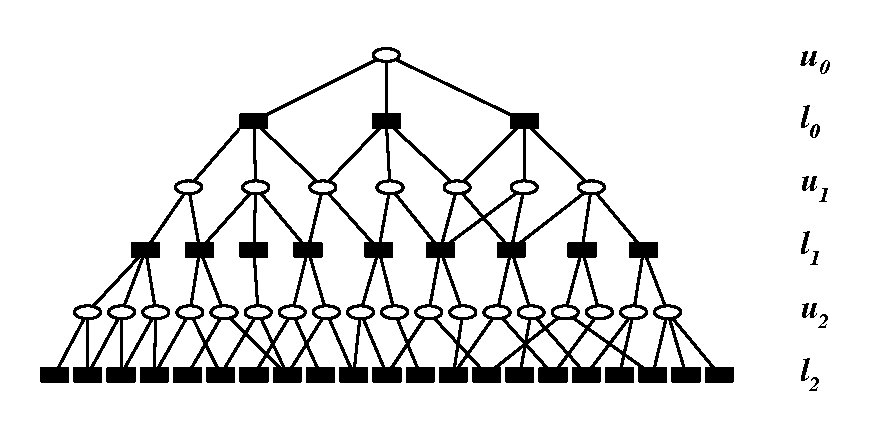
\includegraphics[width=3in]{figures/snowball_sample.eps}
\caption{Schematic of the Snowball Sampling Method}
% JMH to DJW: can we change levels to u_0, l_0, u_1, l_0, etc? (for users @ level 0, lists @ level 0, ...)
\label{fig:snowball_sample_schematic}
\end{figure}

Table~\ref{tab:snowball_sample} shows how many (a) users and (b) lists were
obtained at each level of the snowball sample.  In total, $495,000$ users
were obtained, who appeared on $7,000,000$ lists.  Because users can be
listed in multiple categories (e.g., Oprah Winfrey is frequently included
in lists of ``celebrity'' and ``media''), we next compute a user $u$'s
membership score in category $c$:
\begin{equation}
w_{uc}=\frac{n_{uc}}{N_c},
\end{equation}
where $n_{uc}$ is the number of lists in category $c$ that contain user $u$
and $N_c$ is the total number of lists in category $c$. We then assign each
user to the category in which he or she has the highest membership
score. Users that appear in the follower graph but not in the snowball
sample are assigned to the ``ordinary'' category.


\begin{table}
\centering
\begin{scriptsize}
\caption{Snowball Sample}
\label{tab:snowball_sample}
\begin{tabular}{|c|r|r|r|r|}
\hline
Level 		& celeb	& media & org 	& blog \\ \hline
$u_0$		& 3 	& 2 	& 4		& 32 \\ \hline
$l_0$		& 2342 	& 11403	& 1170 	& 1347 \\ \hline \hline
$u_1$		& 3607 	& 5025 	& 20122	& 16317 \\ \hline
$l_1$		& 30490 & 71605	& 4970 	& 9546 \\ \hline \hline
$u_2$		& 108836 & 309056 & 115034 & 140251 \\ \hline
$l_2$		& 91873 & 171912 & 22518 & 19946 \\ \hline
\end{tabular}
\end{scriptsize}
\end{table}


\subsubsection{Activity Sample of Twitter Lists}
Although the snowball sampling method is convenient and is easily
interpretable with respect to our theoretical motivation, it is also
potentially biased by our particular choice of seeds. To address this
concern, we also generate a sample of users based on their
activity. Specifically, we crawl all lists associated with all users who
tweet at least once every week for the entire observation period.
% DW to SW: Do we retain users who tweet at least once per week, or who
% tweet at least one URL per week?  
% SW: the first case: tweet at least once per week.

This ``activity-based'' sampling method, which yields $750,000$ users and
$5,000,000$ lists (see Table~\ref{tab:sampling-comp} for comparison to the
snowball method), is also clearly biased towards users who are consistently
active. Importantly, however, the bias is likely to be quite different from
any introduced by the snowball sample; thus obtaining similar results from
the two samples should give us confidence that our findings are not
artifacts of the sampling procedure.

%% DW: Refer to Table
%% WM: done
\begin{table}
\centering
\begin{scriptsize}
\begin{tabular}{|c|r|r|r|r|} \hline
 & \multicolumn{2}{|c|} {Snowball Sample} & \multicolumn{2}{|c|} {Activity Sample} \\ \hline
\textit{category} & \# of users & \# of lists & \# of users  & \# of lists\\ \hline
celeb & 108,836 & 91,873 & 22,803 & 68,810 \\ \hline
media & 309,056 & 171,912 & 66,300 & 145,176\\ \hline
org & 115,034 & 22,518 & 19,726 & 16,532\\ \hline
blog & 140,251& 19,946 & 49,987 &17,259\\
\hline
\end{tabular}
\caption{Statistics of crawled lists. The number of users refers only to
  people who appear in at least one list of the specific category.}
\label{tab:sampling-comp}
\end{scriptsize}
\end{table}

% \begin{figure}
% \label{top_k_volume_other}
% \centering
% 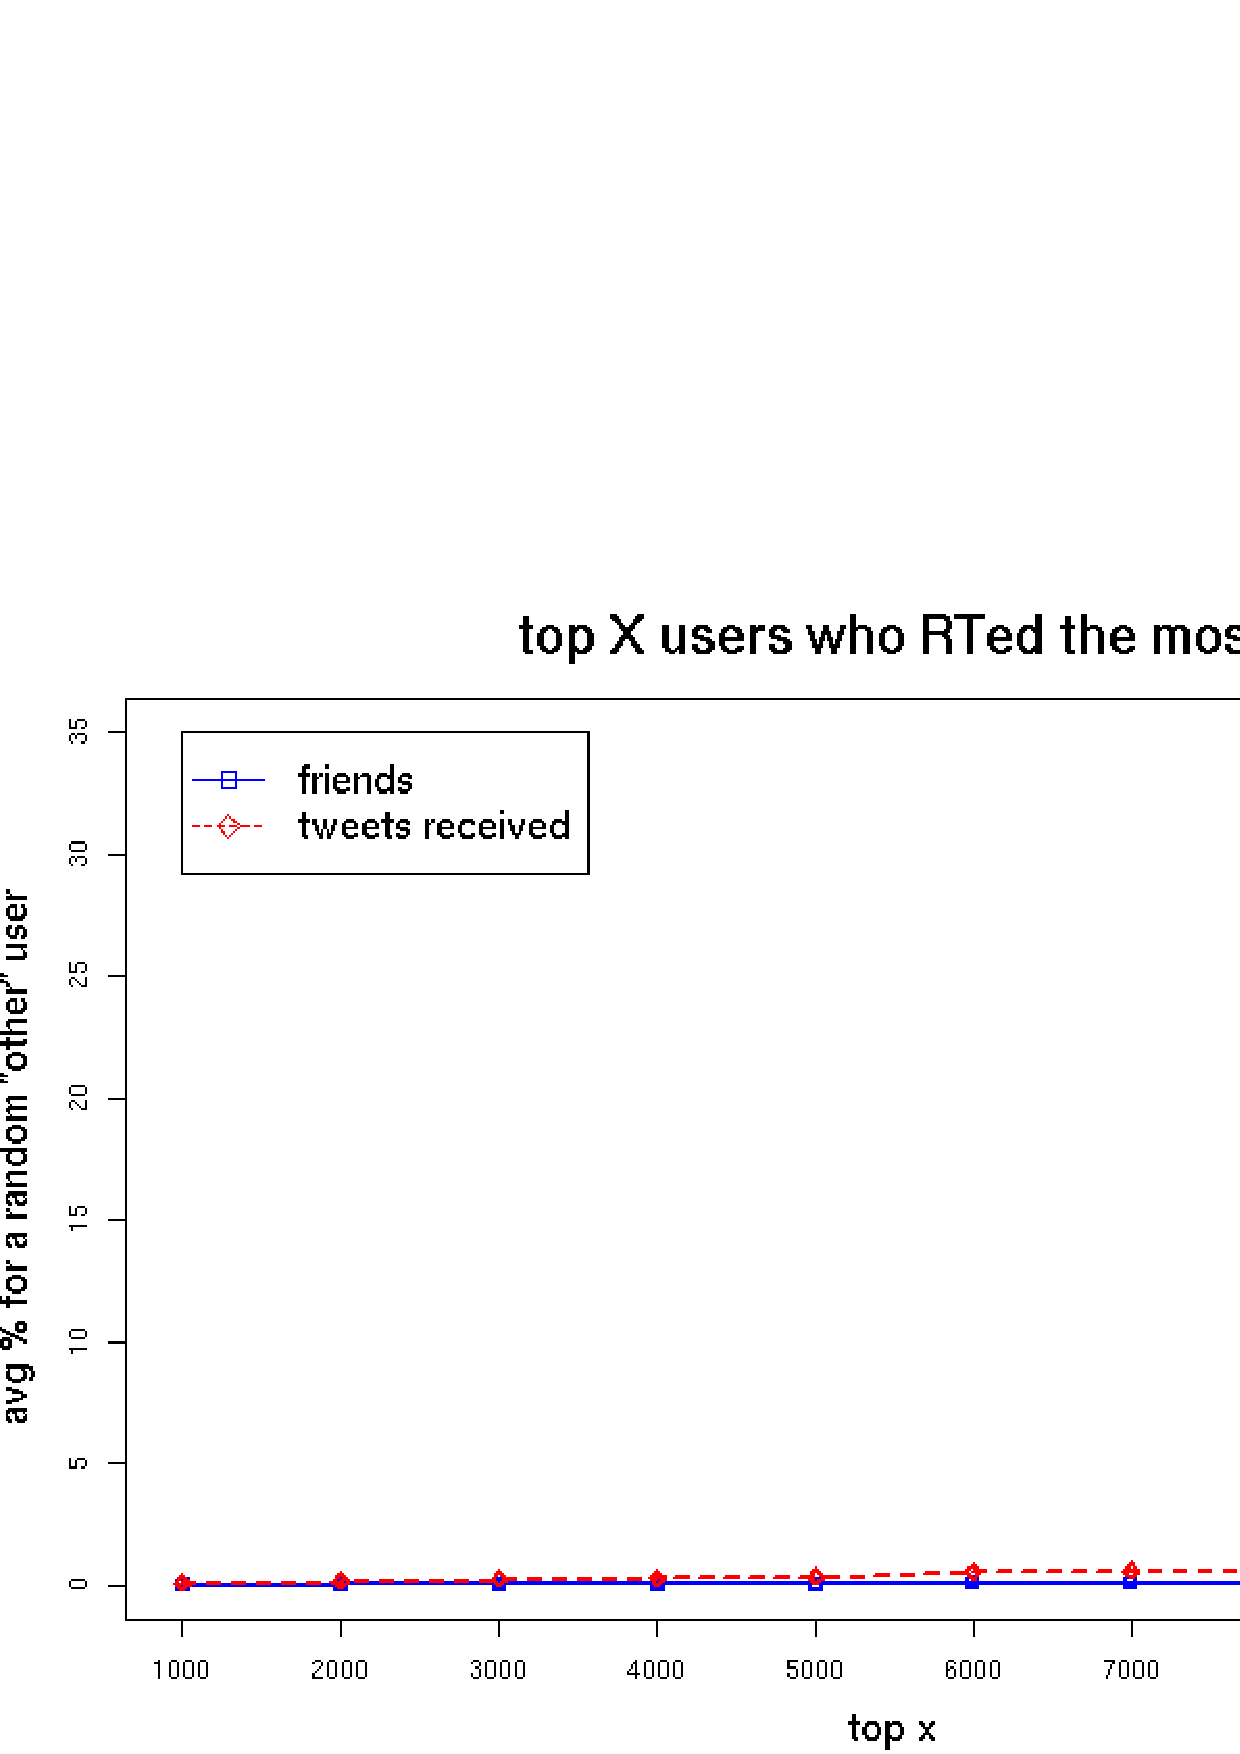
\includegraphics[width=3in]{figures/mostRTing_user_outflow_to_random_other_users.png}
% \caption{}
% \end{figure}

\subsection{Distribution of attention}

After categorizing people into categories, we can calculate the amount of attention sent and received by each category, at a global level. The way we do it is to show the reach of the ``elite'' categories. It can be considered as the influence of each category, as well as an estimate of the impact of the information introducted by each category. In other words, it is the maximal reach of the information produced by each category.



\subsubsection{Concentration of attention}
With either sampling method, the initial categorization of users is quite
coarse and noisy as a result of the arbitrary labeling allowed in Twitter
Lists.  To filter categories to the most representative users, we further
rank the users in each of the 4 elite categories by how frequently they are
listed in each category, and take only the top $k$ users in each category,
relabeling the remainder as ``ordinary'' users. To determine the
appropriate $k$, we measure the flow of information from the four elite
categories to an average ``ordinary'' user in two ways: the proportion of
people the user follows in each category, and the proportion of tweets the
user received from everyone the user follows in each category.  We sampled
100K random ``ordinary'' users and calculated the average information flow
from the ``elite'' users using these two measures.

Figure \ref{fig:attention_elites_snowball} shows that each category
accounts for a significant share of both the following links and also the
tweets received by an average user, where celebrities outrank all other
categories, followed by the media, organizations, and bloggers.  Also of
note is that the bulk of the attention is accounted for by a relatively
small number of users within each category, as evidenced by the relatively
flat slope of the attention curves in Figure
\ref{fig:attention_elites_snowball}. In order to define which users should
be classified as ``elites'', we seek a tradeoff between (a) keeping each
category relatively small, so as not to include users who are not
distinguishable from ordinary users, while (b) maximizing the volume of
attention that is accounted for by each category. In addition, it is also
desirable to make the four categories the same size, so as to facilitate
comparisons.  Balancing these requirements, we therefore choose 5K as a
cut-off for the elite categories.

\begin{figure}[ht]
\centering
\subfigure[Snowball sample]{
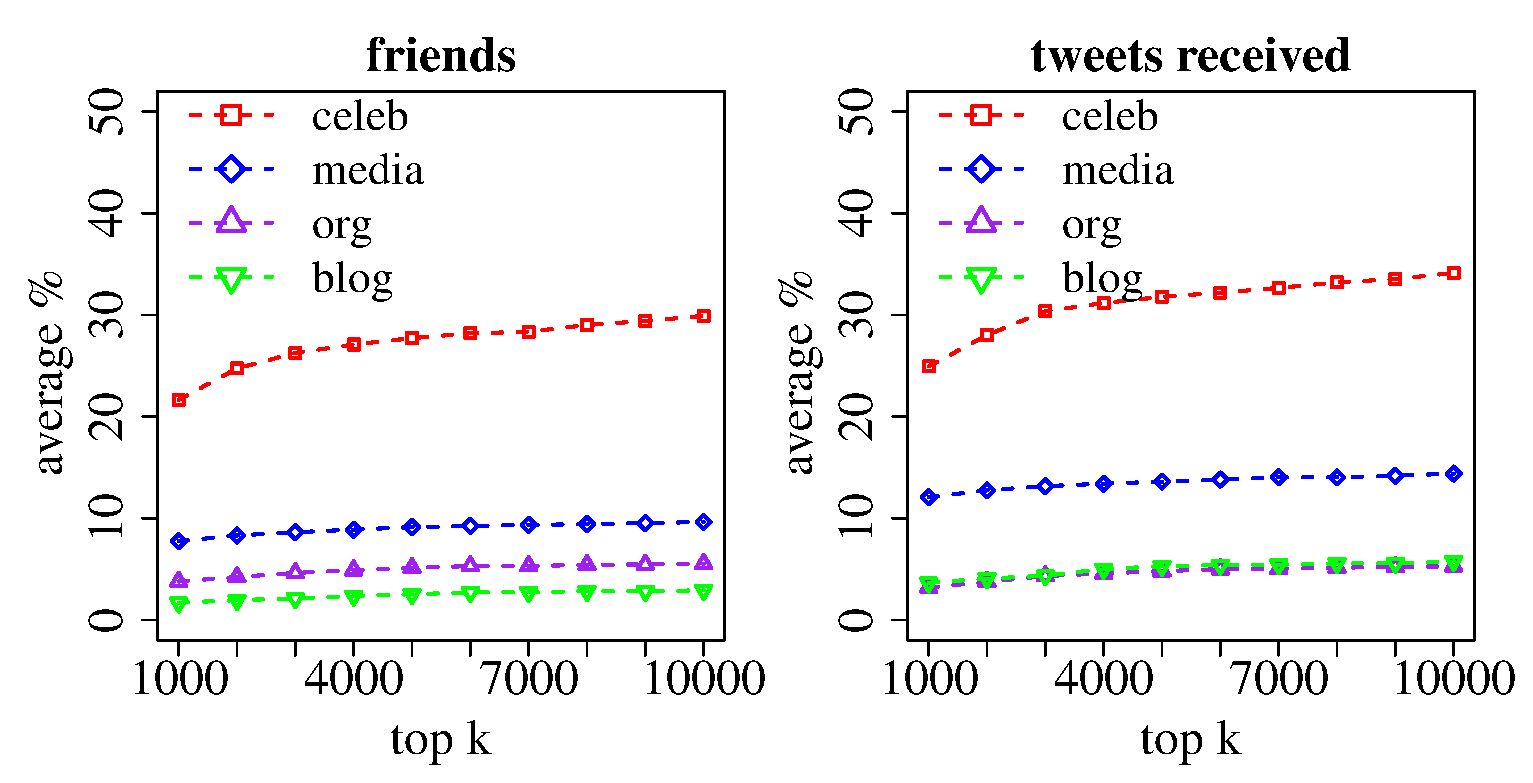
\includegraphics[width=3in]{figures/top_users_outflow_to_random_other_users_500K.eps}
\label{fig:attention_elites_snowball}
}
\subfigure[Activity sample]{
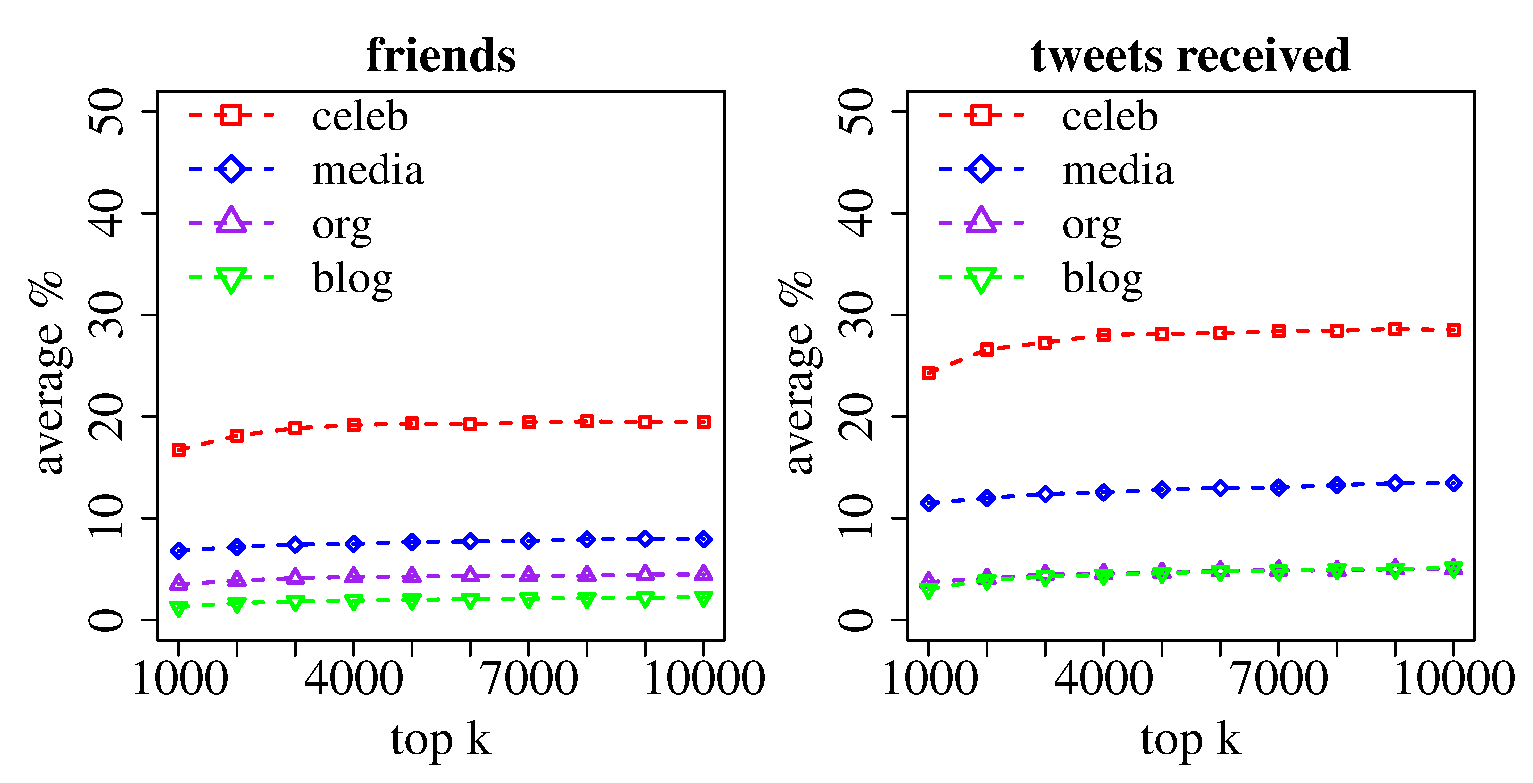
\includegraphics[width=3in]{figures/top_users_outflow_to_random_other_users_800K.eps}
\label{fig:top_k_elite_volume}
}
\label{fig:attention_to_top_k_elite}
\caption{Average fraction of $\#$ following (blue line) and $\#$
  tweets (red line) for a random user that are accounted for by the
  top K elites users crawled}
\end{figure}

%\begin{figure}
%\centering
%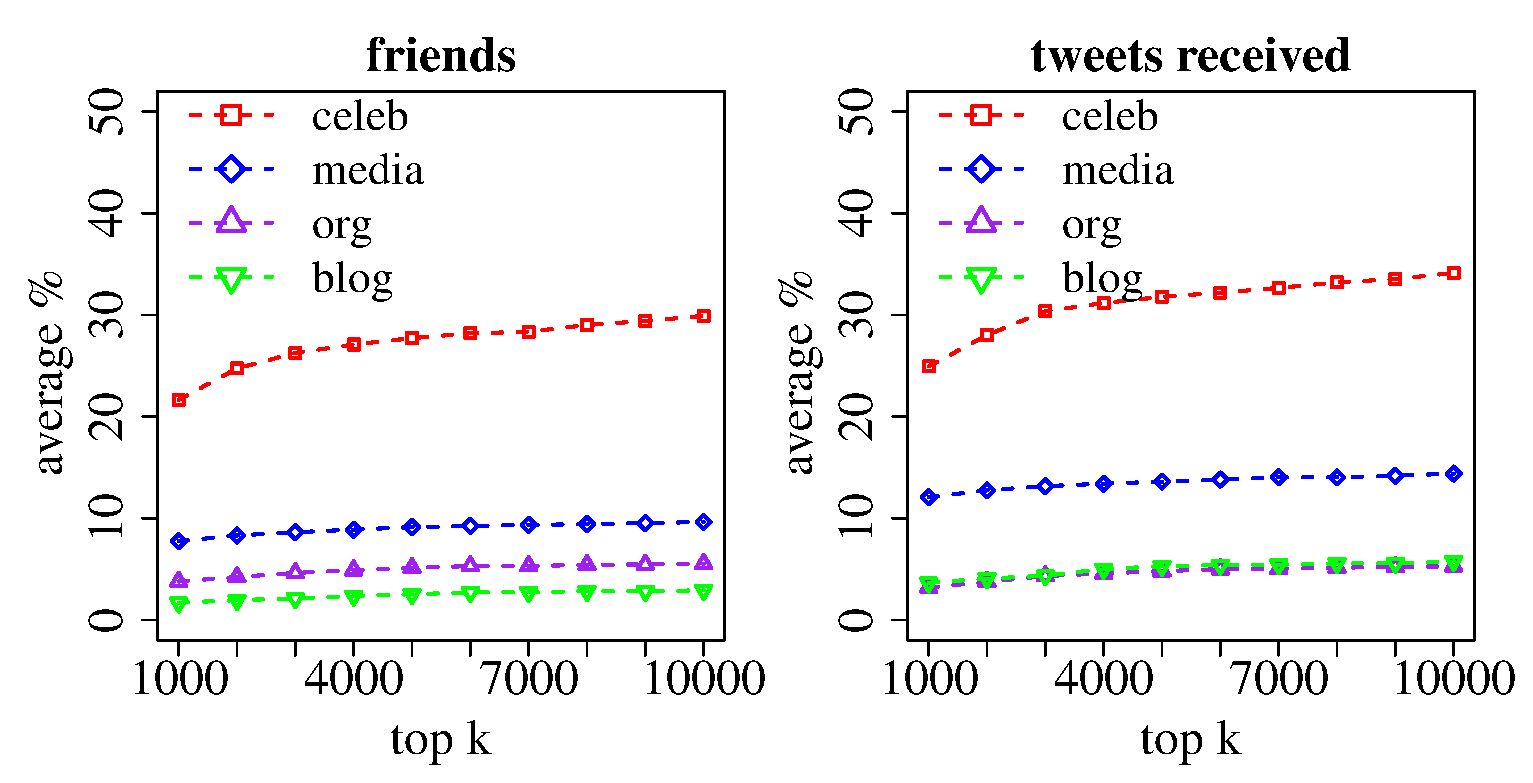
\includegraphics[width=3in]{figures/top_users_outflow_to_random_other_users_500K.eps}
%\caption{Average fraction of $\#$ following (blue line) and $\#$
%  tweets (red line) for a random user that are accounted for by the
%  top K elites users crawled}
%\label{fig:attention_elites_snowball}
%\end{figure}

%\begin{figure}
%\centering
%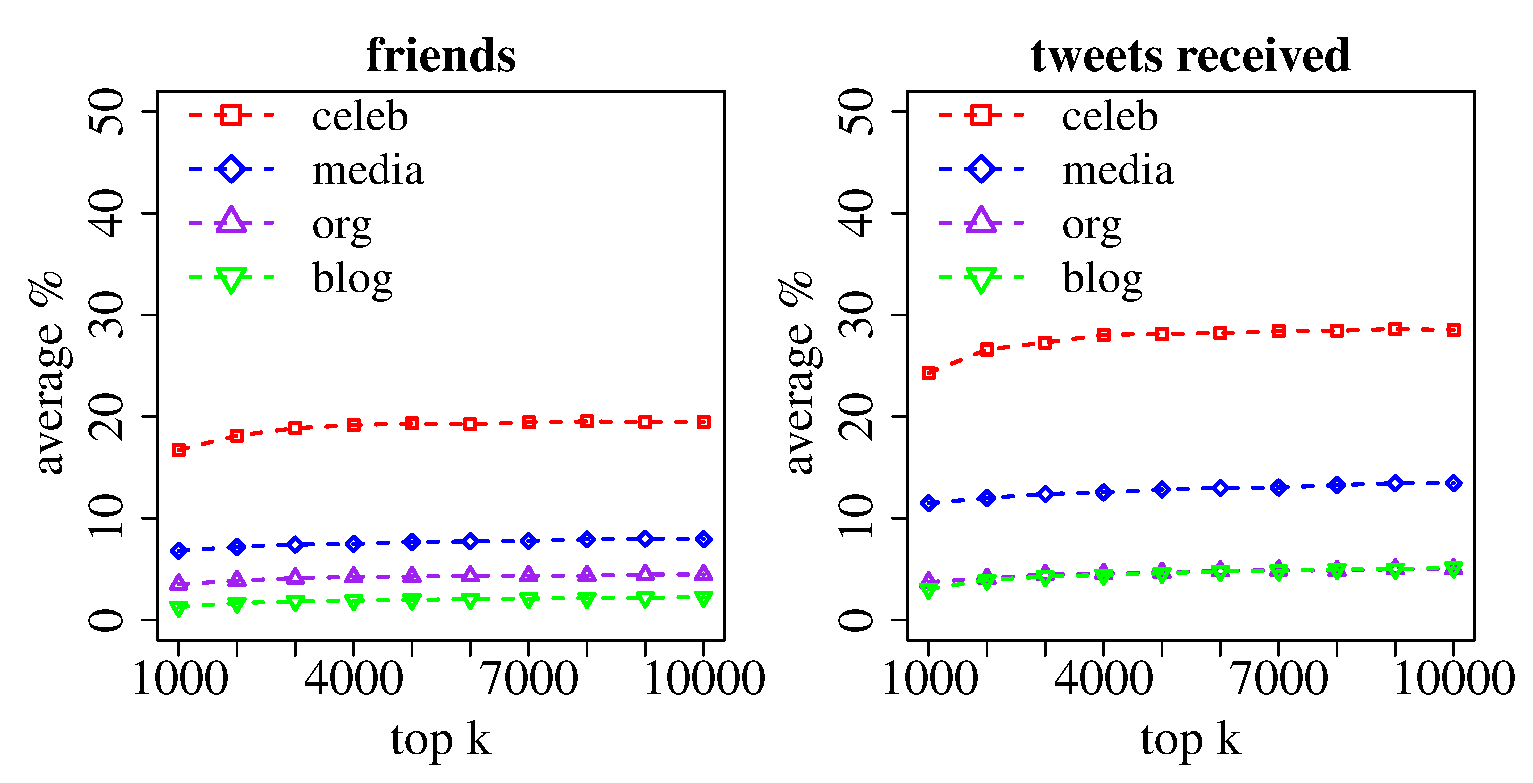
\includegraphics[width=3in]{figures/top_users_outflow_to_random_other_users_800K.eps}
%\caption{Average fraction of $\#$ following (blue line) and $\#$ tweets
%  (red line) for a random user that are accounted for by the top $k$ users
%  classified in one of our four categories}
%\label{fig:top_k_elite_volume}
%\end{figure}


Consistent with this view, we find that the population of users identified
by the activity sample is somewhat different from the snowball sample: the
intersection of the two populations is only 20$\%$ (100,000
accounts). However, the intersection of the top $k$ users in each
population increases as $k$ decreases: for the top $5,000$ users in each
category, the intersection is $41\%$, and for the top $1,000$ users it is
$51\%$. Thus, although the population of consistently active users is
somewhat different from those reached with the snowball sample, the most
frequently listed users in both populations tend to be similar. In
addition, Figure \ref{fig:top_k_elite_volume} shows that the attention paid
to the top $k$ users in the four categories is essentially the same as for
the snowball sample.  Thus in the rest of this paper, when we talk about
``celebrity'', ``media'', ``organization'', ``blog'', we mean the top 5K
users listed as ``celebrity'', ``media'', ``organization'', ``blog'',
respectively, drawn from the snowball sample. Table
\ref{tab:top_k_examples} shows the top 5 users in each of
the four categories.

%  while Figure \ref{top_k_other_volume} reassures us
% that again the unclassified users account for at most a negligible
% fraction of attention.

% JMH to SW: should the axis be adjusted here for better resolution? or
% will this give the false appearance that there's lots of variation wrt x?
% SW: which axis? 

\begin{table}
\centering
\begin{scriptsize}
\caption{Top 5 users in each category}
\vspace{2pt}
\begin{tabular}{|c|c|c|c|} 
\hline 
%\multicolumn{4}{|c|} {Top 5 users} \\ 
%\hline
\textit{Celebrity} & \textit{Media} & \textit{Org} & \textit{Blog} \\ 
\hline
aplusk & cnnbrk & google & mashable \\
ladygaga & nytimes & Starbucks & problogger \\
TheEllenShow & asahi & twitter & kibeloco \\
taylorswift13 & BreakingNews & joinred & naosalvo \\
Oprah & TIME & ollehkt & dooce \\
\hline 
%\multicolumn{4}{|c|} {Bottom 5 users} \\ 
%\hline
%\textit{Celebrity} & \textit{Media} & \textit{Org} & \textit{Blog} \\ 
%\hline
%rajolaurel & singaporenews & worldvisioncan & nicolamattine \\
%wongfupro & TelegraphSci & fujiqnow & machedavvero \\
%FUCKCITY & SZ\_Wirtschaft & KNT\_gakusei & BrideTide \\
%tonyfernandes & TheOaklandPress & overdrive\_jp & theselvedgeyard \\
%Silver90210 & USDOL & ProOkubo & averyps \\
%\hline
\end{tabular}
\label{tab:top_k_examples}
\end{scriptsize}
\end{table}


ZZZZZ: Move the paragraph and tables below to content part.

To confirm the validity of these categories, we now consider the number of
URLs introduced by various categories. As Table \ref{tab:urls_initiated}
(left column) shows, the vast majority of URLs are initiated by ordinary
users, not by any of the elite categories.  This result, however, is
deceptive: as we have just determined, our elite categories number only
$20K$ users in total, whereas we classify over $40M$ users in the
``ordinary'' category.  A more calibrated view is presented in the right
hand column of Table \ref{tab:urls_initiated}, which shows the per-capita
number of URLs originating from various categories.  Here it is clear that
users classified as ``media'' far outproduce all other categories, followed
by bloggers, organizations, and celebrities. In contrast to the previous
result, ordinary users originate on average only about $6$ URLs
each---far fewer than any category of elite users.

%%DW: Need to note at some point in this section that from now on we will
%%use snowball sample; all results are the same.
%%WM: done, in previous paragraph

% JMH: Need to add a second column for per-capita initiations.
% WM: done
\begin{table}
\centering
\caption{\# of URLs initiated by category}
\label{tab:urls_initiated}
\begin{tabular}{l r r}
\textit{category} & \# of URLs & per-capita \# of URLs \\ 
\hline
celeb	& 139,058 & 27.81 \\ 
media	& 5,119,739 & 1023.94 \\ 
org	& 523,698 & 104.74 \\ 
blog	& 1,360,131 & 272.03 \\ 
other	& 244,228,364 & 6.10\\
\end{tabular}
\end{table}


Conceivably, our classification scheme above has omitted an important
category; that is, within the current ``other'' category may be hidden
additional categories of opinions.  As Figure \ref{top_k_volume_other}
shows, however, even the top 10,000 most followed of these users
accounts for a negligible fraction of attention among the remaining
population.  
 
\begin{figure}
\label{top_k_volume_other}
\centering
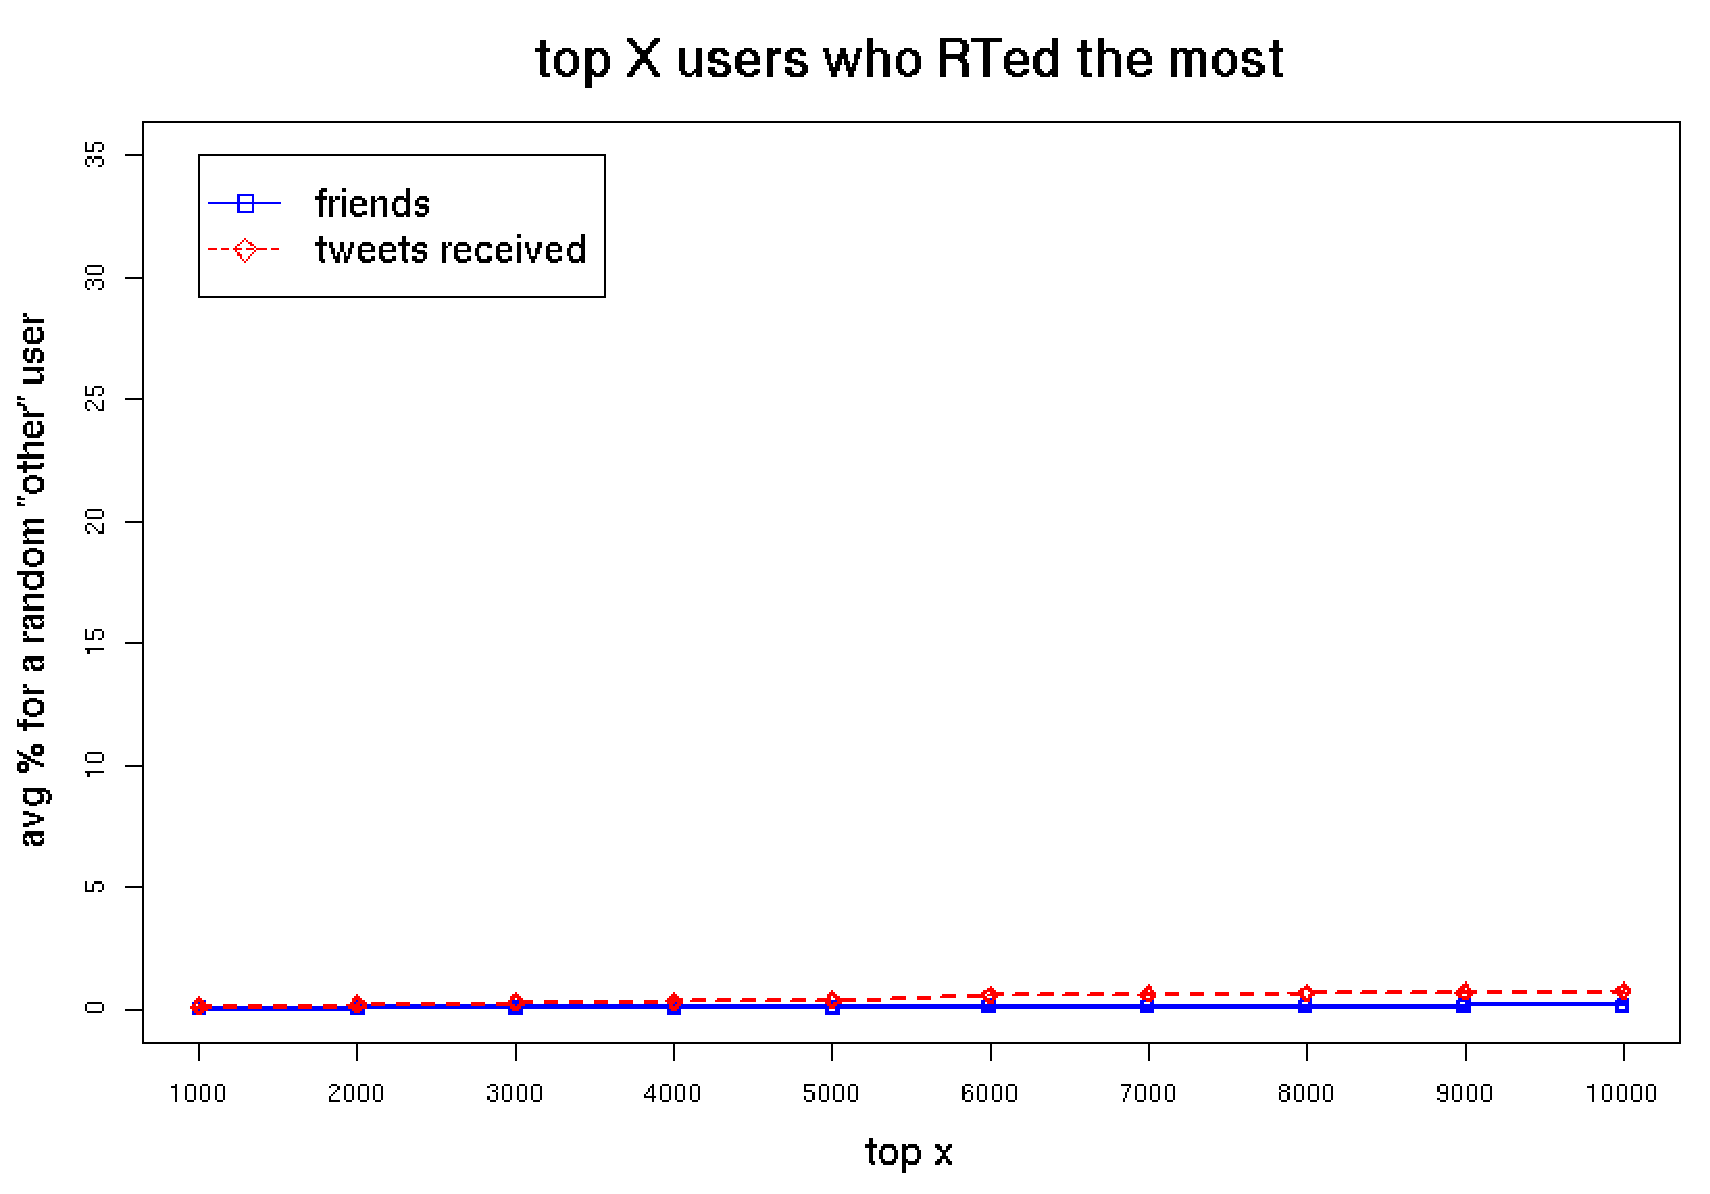
\includegraphics[width=3in]{figures/mostRTing_user_outflow_to_random_other_users.eps}
\caption{Average fraction of $\#$ following (blue line) and $\#$
  tweets (red line) for a random user that are accounted for by the
  top K most retweeted users in the ``Other'' category}
\end{figure}


\subsubsection{Homophily of attention}

As indicated above, the top $20K$ elite users account for almost $50 \%$ of
all attention within Twitter; yet this population of users comprises less
than $0.05\%$ of the population.
% As we can see in Figure \ref{fig:topuser_to_other}, for an ordinary
% Twitter user, a significant portion of people he follows are among the
% small number of ``elite'' users we identified, and an even higher
% portion of the tweets he receives are directly from those elite users.
In other words, although Twitter clearly reflects the conventional wisdom
that audiences have become increasingly fragmented, it nevertheless shows
remarkable concentration of information production and received attention
among a relatively small number of actors. Even if the media has lost
attention relative to other elites, information flows have not become
egalitarian by any means.

The prominence of elite users raises the question of how these different
categories listen to each other.  To address this issue, we compute the
percentage of following links and received tweets among elite
categories. Specifically, Table \ref{tab:flow_among_categories} shows the
average percentage of friends/tweets category $i$ get from category
$j$. Table \ref{tab:flow_among_categories} shows striking homophily with
respect to attention: celebrities overwhelmingly pay attention to other
celebrities, media actors pay attention to other media actors, and so on.
The one slight exception to this rule is that organizations pay more attention
to bloggers than to themselves.  In general, in fact,
attention paid by organizations is more evenly distributed across
categories than for any other category.

\begin{table}
\centering
\begin{scriptsize}
\caption{Information flow among the elite categories}
\label{tab:flow_among_categories}
\vspace{2pt}
\begin{tabular}{|c|r|r|r|r|}
\hline
\% of friends &	in celeb  &	in media &	in org	& in blog \\\hline
celeb	& \bf{30.56} & 3.63 & 1.99 & 1.64 \\ \hline
media	& 3.59 & \bf{16.67} & 2.07 & 2.15 \\ \hline
org	& 3.62 & 3.33 &	\bf{7.38} & 2.65 \\ \hline
blog	& 4.41 & 2.27 &	2.03 &	\bf{10.25} \\ \hline
\hline
\% of tweets &	from celeb	&from media	&from org	&from blog \\ \hline
celeb	& \bf{38.27} & 6.23 & 1.55 & 3.98\\ \hline
media	&3.91 & \bf{26.22} & 1.66 & 5.69 \\ \hline
org	&4.64 & 6.41 &	8.05 & \bf{8.70} \\ \hline
blog	&4.94 & 3.89 & 1.58 & \bf{22.55} \\ \hline
\end{tabular}
\end{scriptsize}
\end{table}

\begin{figure}
\centering
\includegraphics[width=3in]{figures/visualization_500K_tweets.eps}
\caption{Share of attention among elite categories}
\label{fig:topuser_to_other}
\end{figure}



\section{ZZZZZ: Transmissive probability}
ZZZZZ: should we combine this section with previous or next section?

For information that do spread, most previous works study the factors that contribute to the spread at each hop, independently. (ZZZZZ related work).

The categorization of actors, as introduced previously, also helped shed some light on the one-hop diffusion probability, depending on the type of users in the diffusion edge, and people's interest at different types of content.

My contribution:
\begin{enumerate}
\item Show homophily at diffusion;
\item Show difference in attention and influence (as measured by RTs)
\item Show people's interest at different content.
\end{enumerate}

\subsection*{People}
The origin of information will influence how it will be RTed.
 
Before proceeding, it is helpful to differentiate between two mechanisms by
which information can diffuse in Twitter. The first is via retweeting, when
a user, having received a tweet, subsequently rebroadcasts it to his or her
own followers. In some instances, users retweet each other using the
official retweet function provided by Twitter, but in other cases they
credit the retweet with an informal convention, most commonly either ``RT
@user" or ``via @user.'' The second mechanism is what we label
reintroduction, where a user independently tweets a URL that has previously
been introduced by another user.
%\footnote{Because users do sometimes retweet other users without
%  acknowledgement, we have likely misclassified some fraction of retweets
%  as reintroductions. One way to address this issue would be to count as a
%  retweet any appearance of a URL that had previously been tweeted by a
%  user that the current user is following. However, this solution raises
%  additional problems, and in any case does not occur sufficiently
%  frequently to affect our results; thus we treat all reappearances of a
%  URL as reintroductions unless specifically acknowledged as a retweet.}.

In addition to attention, Table \ref{tab:rt_breakdown} shows how much
information originating from each category is retweeted by other
categories, while Table \ref{tab:reintro_breakdown} shows how much is
subsequently reintroduced.  As with attention, both retweeting and
reintroduction activities are strongly homophilous among elite categories;
however, bloggers are disproportionately responsible for retweeting and
reintroducing URLs originated by all categories. This result reflects the
characterization of bloggers as recyclers and filters of information;
however, Table \ref{tab:rt_breakdown} and \ref{tab:reintro_breakdown} also
show that the total number of URLs either RT'd or reintroduced by bloggers
is vastly outweighed by the number retweeted or reintroduced by ordinary
users.  Even though on a per-capita basis, therefore, bloggers
disproportionately occupy the role of information recyclers, their actual
impact is relatively minimal (see Figure \ref{fig:topuser_to_other}).

\begin{table*}
\centering
\caption{RTs among categories}
\label{tab:rt_breakdown}
\begin{tabular}{|l|r|r|r|r|r|r|}
\hline
 &  by celeb & by media & by org & by blog & by other & TOTAL\\ \hline
celeb & 4,334 & 1,489 &	1,543 &	5,039 &	1,070,318  & 1,082,723\\ \hline
media & 4,624 & 40,263 & 7,628&32,027 & 5,204,719  & 5,289,261\\ \hline
org & 1,570 & 2,539 & 18,937 & 11,175 & 1,479,017 & 1,513,238\\ \hline
blog & 3,710 & 6,382 & 5,762 & 99,818 & 3,457,631 & 3,573,303\\ \hline
other & 34,455 & 93,934 & 86,630 & 318,537 & 34,814,456 & 35,348,012\\ \hline
\end{tabular}
\end{table*}

\begin{table*}
\centering
\caption{Re-introductions among categories}
\label{tab:reintro_breakdown}
\begin{tabular}{|l|r|r|r|r|r|r|}
\hline
& by celeb & by media & by org & by blog & by other & TOTAL\\ \hline
celeb &	2,868 & 1,239 & 522 & 1,664 & 488,229 & 494,522\\ \hline
media & 1,678 & 205,165 & 2,439	& 9,681	& 2,006,888 & 2,225,851\\ \hline
org & 816 & 1,511 & 8,628 & 3,711 & 610,373 & 625,039\\ \hline
blog & 1,415	& 5,644	& 1,416	& 52,909 & 1,148,137 & 1,209,521\\ \hline
other & 45,547 & 793,741 & 69,441 & 335,690 & 86,853,224 & 88,097,643\\ \hline
\end{tabular}
\end{table*}

\begin{figure}
\centering
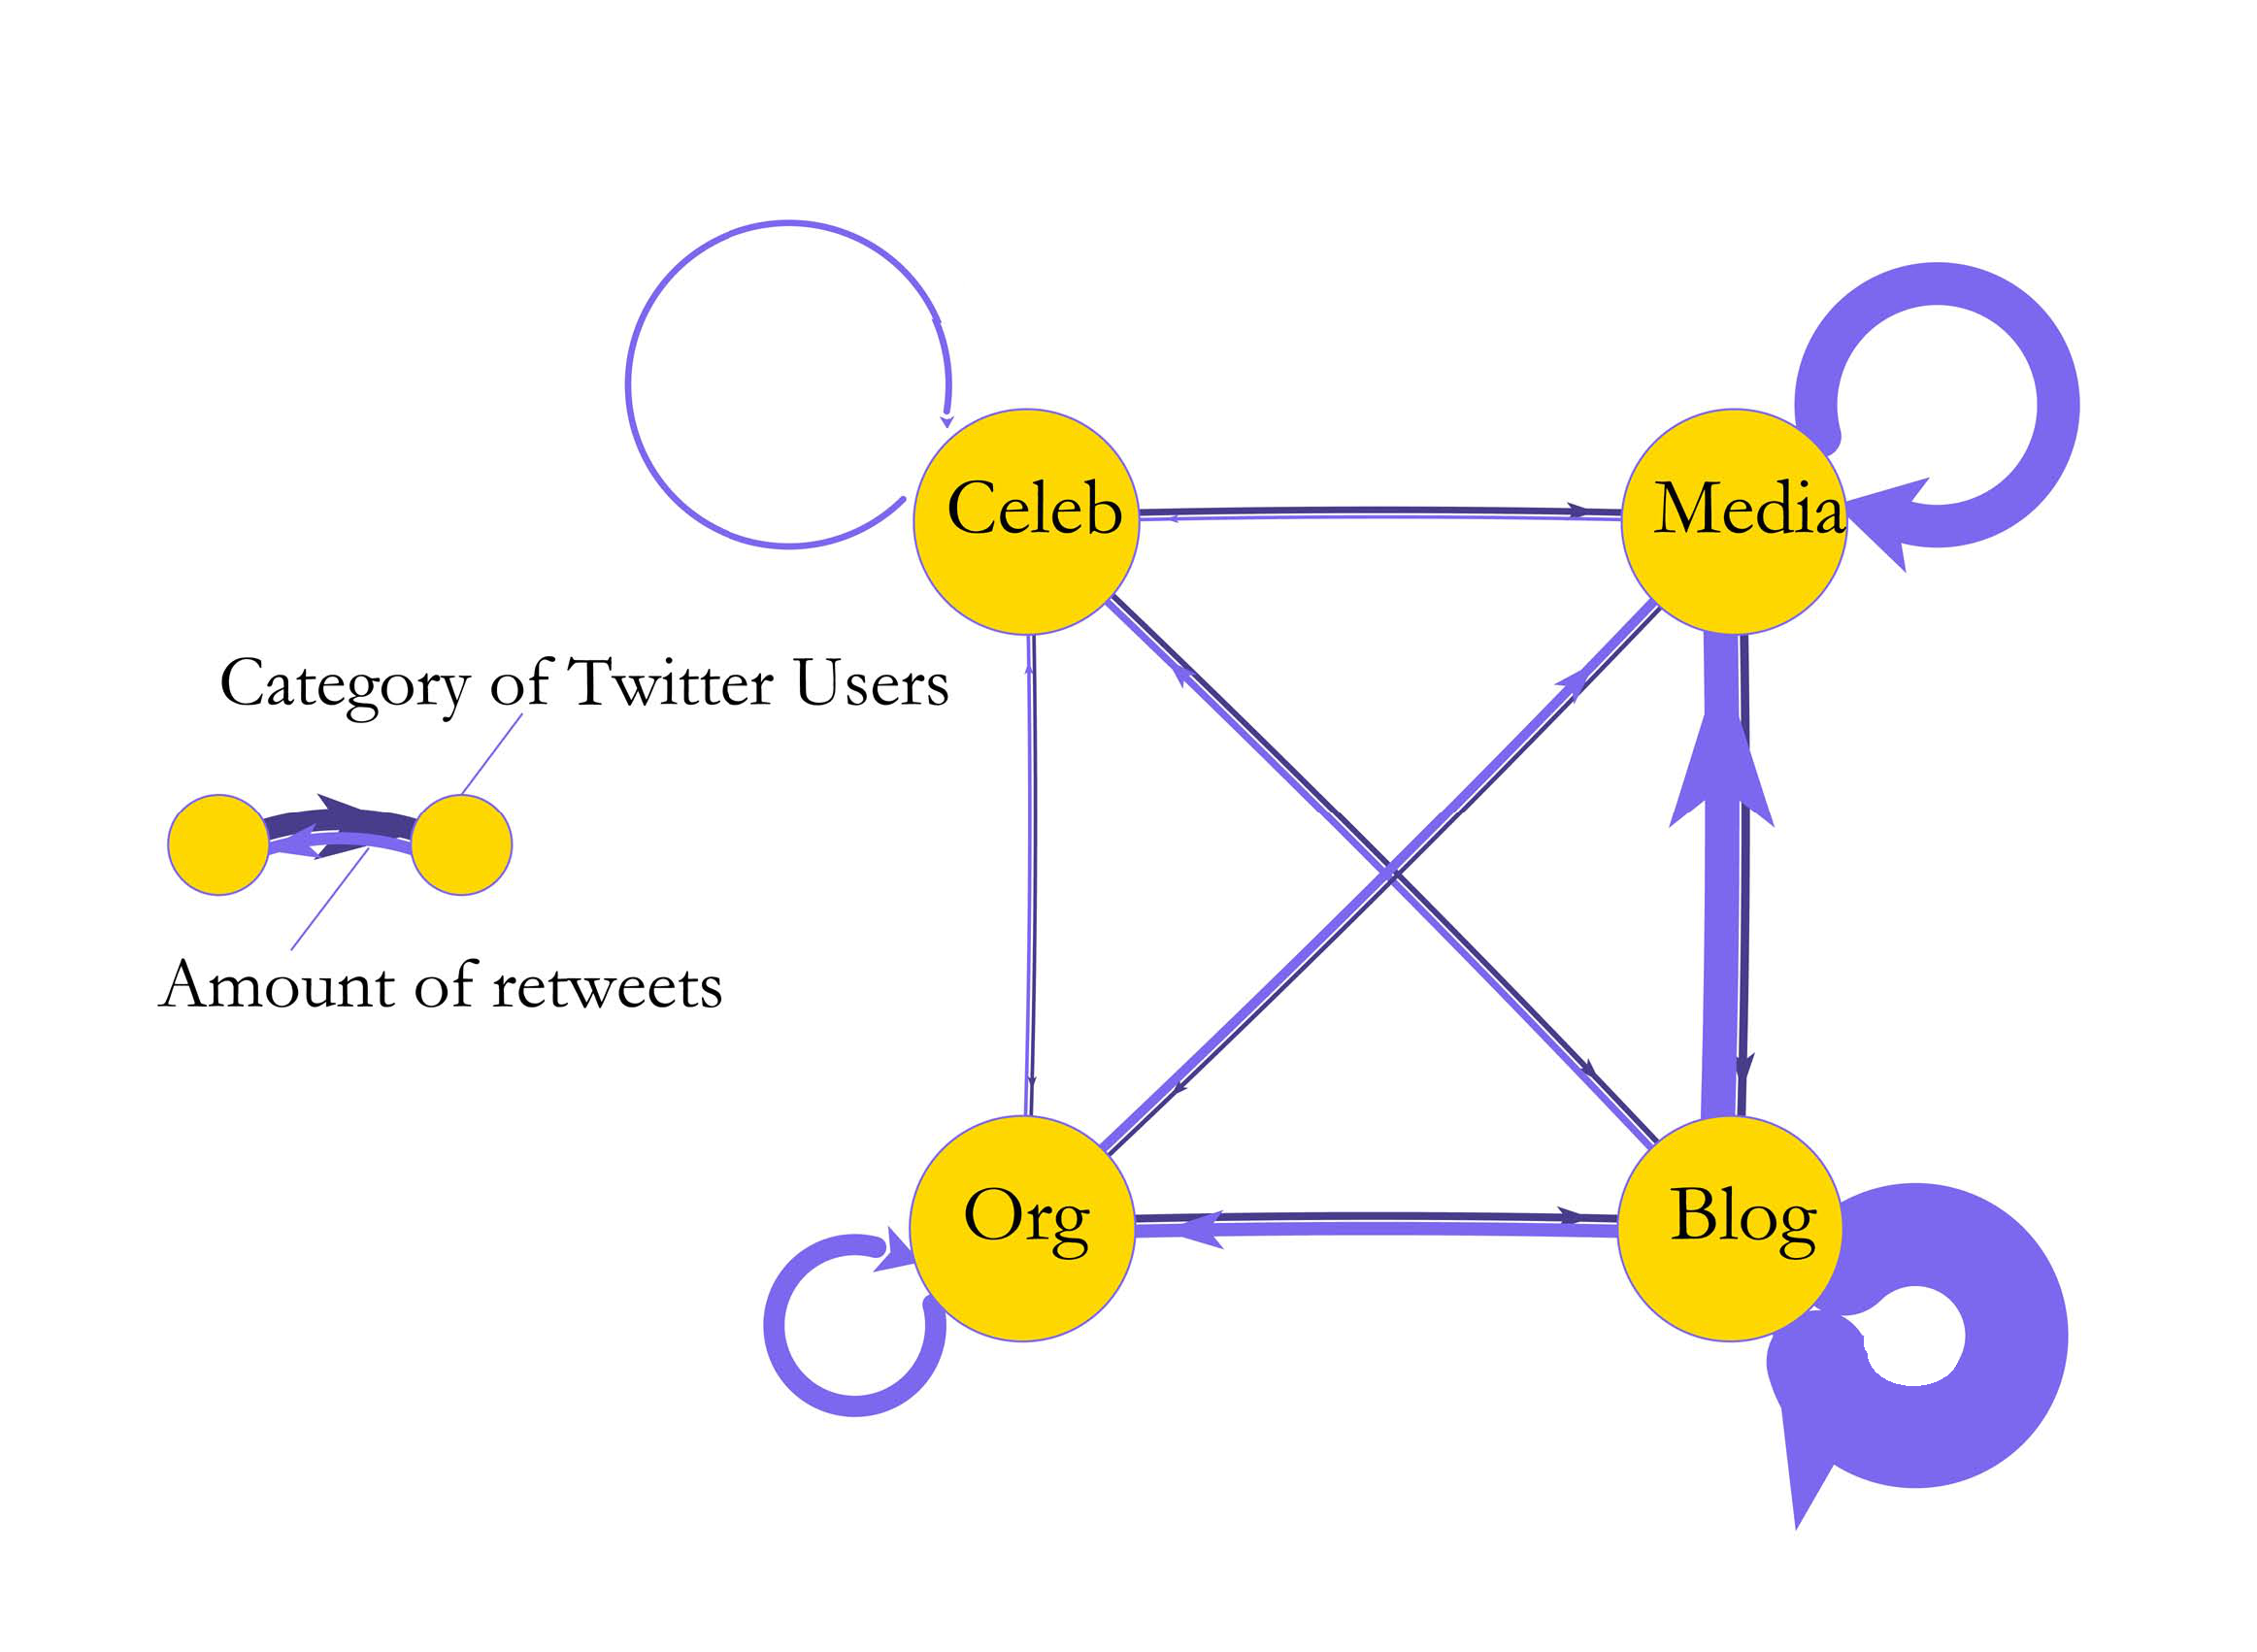
\includegraphics[width=3in]{figures/rt_topUsers_500K.eps}
\caption{RT behavior among elite categories}
\label{fig:RT_topuser}
\end{figure}

\subsection{Content}
People have different interest at different content. So the type of content can also determine what a person will RT.

Given the large size of the URL population in our observation period
($260M$), and the large number of ways in which one can classify content
(video vs. text, news vs. entertainment, political news vs. sports news,
etc.), classifying even a small fraction of URLs according to content is an
onerous task. Bakshy et al \cite{bakshy_11}, for example, used Amazon's
Mechanical Turk to classify a stratified sample of 1,000 URLs along a
variety of dimensions; however, this method does not scale well to larger
sample sizes.

Instead, we restrict attention to URLs originated by the New York Times
which, with over 2.5M followers, is the second-most followed news
organization on Twitter after CNN Breaking News. NY Times, however, is
roughly ten times as active as CNN Breaking News, so is a better source of
data. To classify NY Times content, we exploit a convenient feature of
their format---namely that all NY Times URLs are classified in a consistent
way by the section in which they appear (e.g. US, World, Sports, Science,
Arts, etc)
~\footnote{http://www.nytimes.com/year/month/day/category/\\title.html?ref=category}.
Of the 6398 New York Times bit.ly URLs observed, 6370 could be successfully
unshortened and assigned to one of 21 categories. Of these, however, only 9
categories had more than 100 URLs over the observation period, one of
which---``NY region''---was highly specific to the New York metropolitan
area; thus we focused our attention on the remaining 8 topical categories.
Figure \ref{fig:nytimes_categories} shows the overall RT and reintroduction
rates by category. World news is the most popular category, followed by US
news, business, and sports, where increasingly niche categories like
Health, Arts, Science, and Technology are less popular still.  In general,
the overall pattern is replicated for all categories of users, but there
are some minor deviations: In particular, organizations show
disproportionately little interest in business and arts-related stories,
and disproportionately high interest in science, technology, and possibly
world news. Celebrities, by contrast, show greater interest in sports and
less interest in health, while the media shows somewhat greater interest in
US news stories.

% ======= 
% Instead, we adopt a more limited approach. First, we restrict attention
% to URLs originated by one of just two major news organizations, the New
% York Times and CNN; and second, after unshortening all such URLs, we
% exploit a convenient feature of their format---namely that all such URLs
% are classified in a consistent way by the section in which they appear
% (e.g. US, World, Sports, Science, Arts, etc).  For example, all New York
% Times URLs that appear in the business section have the format:
% http://www.nytimes.com/XXXX/XX/XX/business/123abc.html?ref=business,
% while CNN has an analogous structure; thus it is a trivial matter to
% associate all 6,398 NYTimes and 1,804 CNN URLs with the corresponding
% topic section.

\begin{figure}
\centering
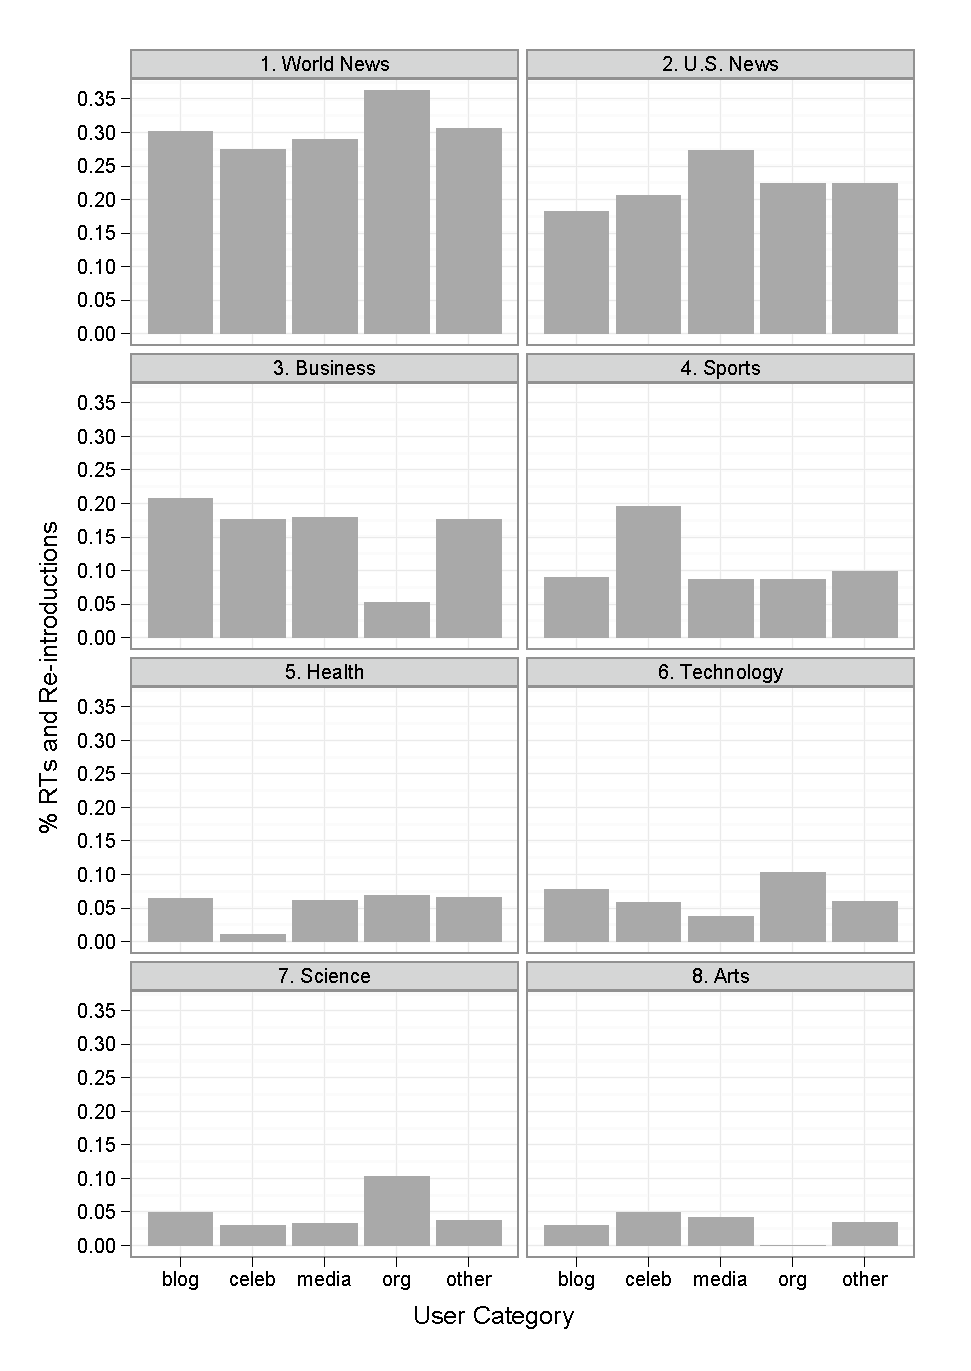
\includegraphics[width=3in]{figures/nyt_url_cat.eps}
\caption{Number of RT's and Reintroductions of New York Times stories by content category}
\label{fig:nytimes_categories}
\end{figure}

In addition, we also consider the accumulated RT/Reintroduction behavior for a
small selection of the most popular URLs. As Figure \ref{fig:popular_URLs}
shows, the link to the official White House blog, which expressed the
administration's initial response to the Haiti earthquake, was rebroadcast
in largely the same manner by all categories of users, as was the
announcement of President Obama winning the Nobel Peace Prize.  By
contrast, the news story announcing the unexpected death of the actress
Brittany Murphy was rebroadcast largely by bloggers, while the breaking
news about Tiger Woods' accident and affair was picked up mostly by the
news media and other celebrities.  Finally, Figure \ref{fig:popular_URLs}
shows two examples of URLs that exhibit very different patterns from news
stories.  First, the URL for DealPlus, a website for ``finding, discussing,
and sharing thousands of deals and coupons for all types of stores,'' was
popular among ordinary users, but almost completely ignored by all
categories of elite users. And second, the video for the song ``Brick by
Boring Brick," by the band Paramore, was again reposted mostly by ordinary
users, but in this case celebrities also reposted it.  Although this
analysis is far from systematic, it suggests that different categories of
users respond to different sorts of content in ways that are consistent
with our classification scheme.

\begin{figure}
\centering
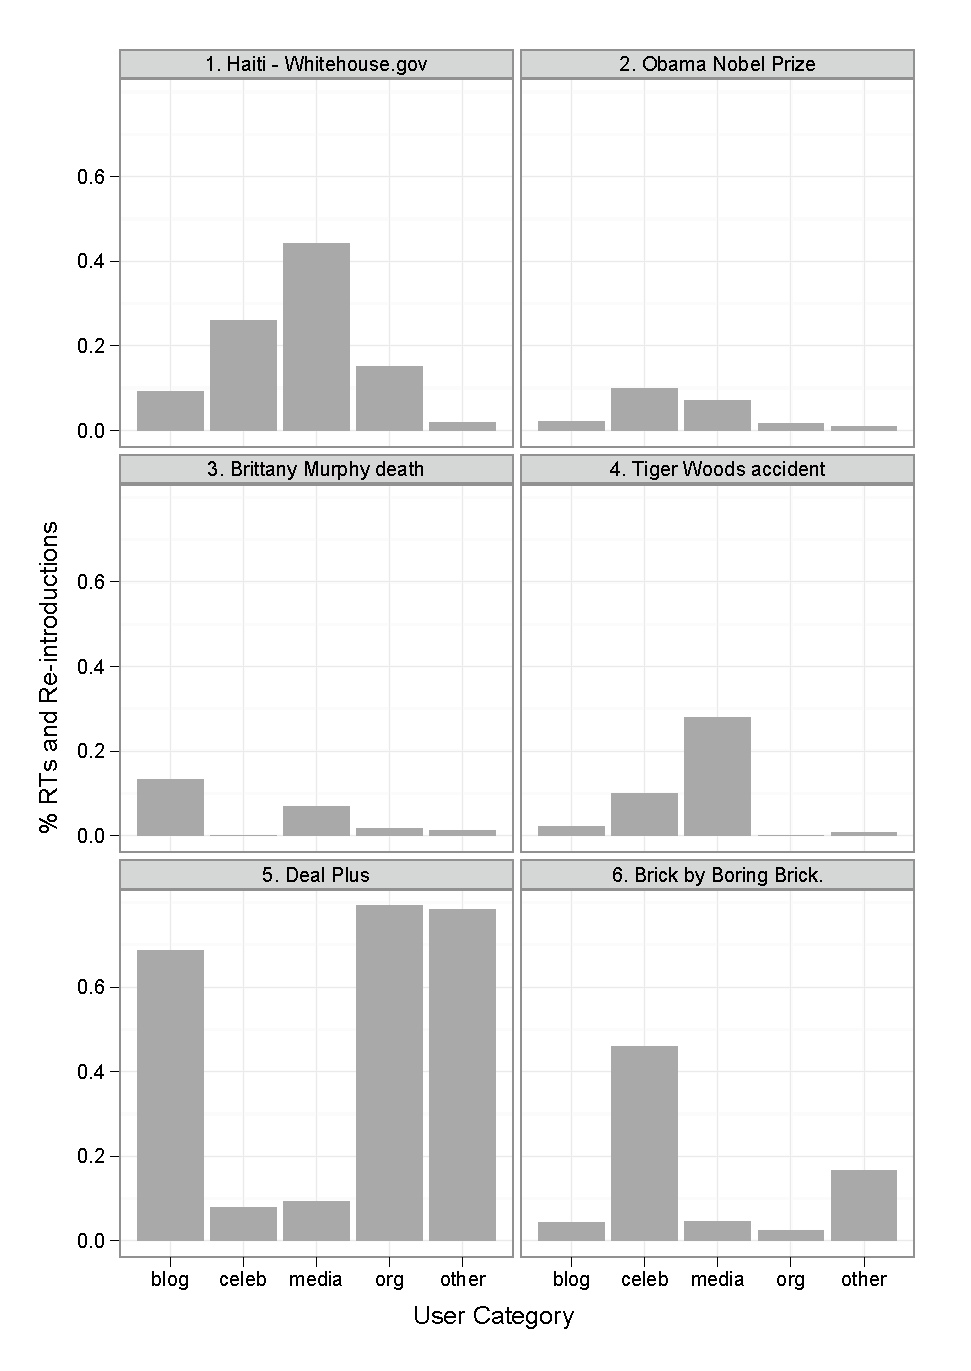
\includegraphics[width=3in]{figures/pop_url_cat_RT.eps}
\caption{Number of RT's and Reintroductions of most popular URLs originating from media and other}
\label{fig:popular_URLs}
\end{figure}



\section{Persistence of information}
In our work, we noticed that although a small amount of information spread and travels, among them, a substantial portion has a very long lifespan. We think this is very interesting phenomenon that has not been well investigated yet. 


\subsection{Lifespan by the category of originator}
ZZZZZ: Content produced by different people have different persistence. Blogger's role of information filter.

By lifetime, we mean the time lag between the first and last
appearance of a given URL on Twitter. Naively, measuring lifetime seems a
trivial matter; however, it is complicated by the finite observation
window, which results in ``censoring'' of our data. In other words, a URL
that is last observed towards the end of the observation period may be
retweeted or reintroduced after the period ends, while correspondingly, a
URL that is first observed toward the beginning of the observation window
may in fact have been introduced before the window began. What we observe
as the lifetime of a URL, in other words, is in reality a lower bound on
the lifetime. Although this limitation does not create much of a problem
for short-lived URLs---which account for the vast majority of our
observations---it does create large biases for long lived URLs. In
particular, URLs that appear towards the end of our observation period will
be systematically classified as shorter-lived than URLs that appear towards
the beginning.

To address the censoring problem, we seek to determine a buffer $\delta$ at
both the beginning and the end of our $223$ day period, and only count URLs
as having a lifetime of $\tau$ if (a) they do not appear in the first
$\delta$ days, (b) they first appear in the interval between the buffers,
and (c) they do not appear in the last $\delta$ days.  As Figure
\ref{fig:censoring} shows, to determine $\delta$ we first split the $223$
day period into two segments - the first 133 day training segment and the last 90 day testing segment, and then ask: if we (a) observe a URL first appear in
the first $163 - \delta$ days and (b) do not see it in the $\delta$
days prior to the splitting point, how likely are we see it in the last 90 days?
Clearly this depends on the actual lifetime of the URL, where initially we
know for each URL that it persists for at least $\tau$ days. As the longer a URL lives, the more likely it will re-appear in the future, Figure
\ref{fig:tau_v_delta} shows the upper-bound on lifetime for which we
can determine the actual lifetime with $95 \%$ accuracy as a function of
$\delta$. Finally, because we require a beginning and ending buffer, and
because we can only classify a URL as having lifetime $\tau$ if it
appears at least $\tau$ days before the end of our window, we need to pick
$\tau$ and $\delta$ such that $\tau + 2\delta < 223$. From Figure
\ref{fig:tau_v_delta}, we determined that $\tau = 60$ and $\delta=48$
sufficiently satisfy our constraints.

%%DW: Insert Figures: (a) schematic of window estimation procedure; (b) tau vs delta tau

%%SW: done

\begin{figure}
\centering
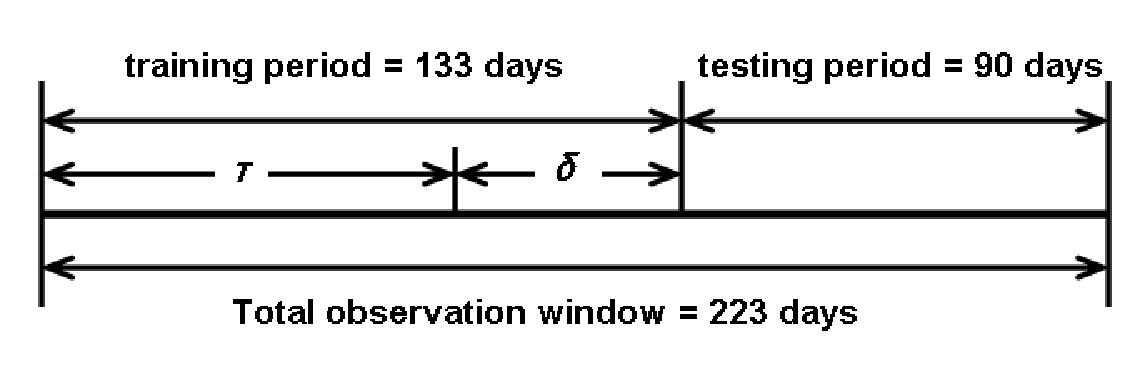
\includegraphics[width=3in]{figures/window_estimation_procedure_scheme.eps}
\caption{Schematic of window estimation procedure}
\label{fig:censoring}
\end{figure}

\begin{figure}
\centering
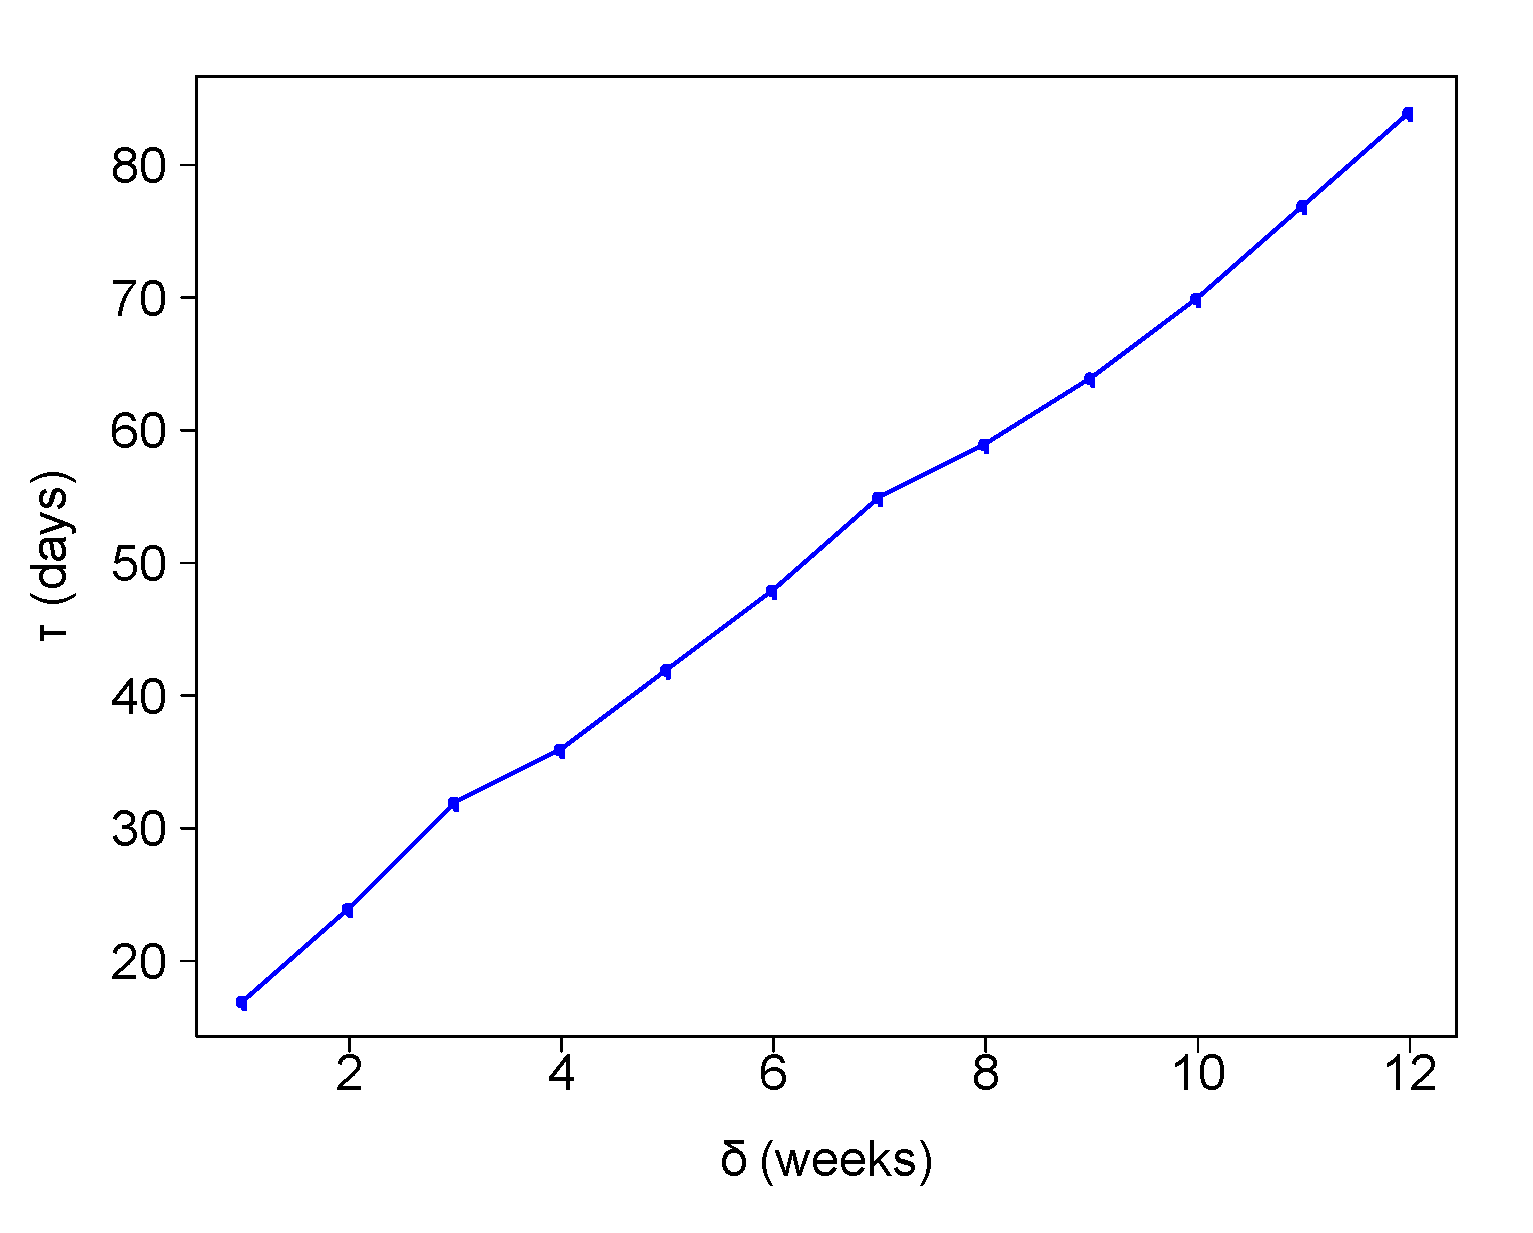
\includegraphics[width=3in]{figures/tau_delta.eps}
\caption{Upperbound of $\tau$ with confidence level > 0.95, as a function of $\delta$.}
\label{fig:tau_v_delta}
\end{figure}


ZZZZZ: some of the numbers here should be move above!!!

Figure \ref{fig:lifespan_category} is the histogram of the lifespan of
URLs, grouped by the category of users who introduced the
URLs\footnote{This figure only shows URLs that appeared in our dataset more
than once.  The majority of the URLs (220M) appeared only once, which is 10
times as many URLs as had a lifespan of only a day.}.  
%
URLs initiated by the elite categories exhibit a similar distribution over
lifespan to those initiated by ordinary users. As Figure
\ref{fig:lifespan_percentage_category} shows, however, when looking at the
percentage of URLs of different lifespans initiated by each category,
we see two additional results: first, URLs originated by media actors
generate a large portion of short-lived URLs (especially URLs with
lifespan 0, which are URLs that only appeared once); and second, URLs
originated by bloggers are overrepresented among the longer-lived content.
Both these results can be accounted for by the type of content
that originates from different sources: whereas news stories tend to be
replaced by updates on a daily or more frequent basis, the sorts of
stories that are picked up by bloggers are of more persistent interest, and
so are more likely to be RT'd or reintroduced months or even years after
their initial introduction.


\begin{figure}
\centering
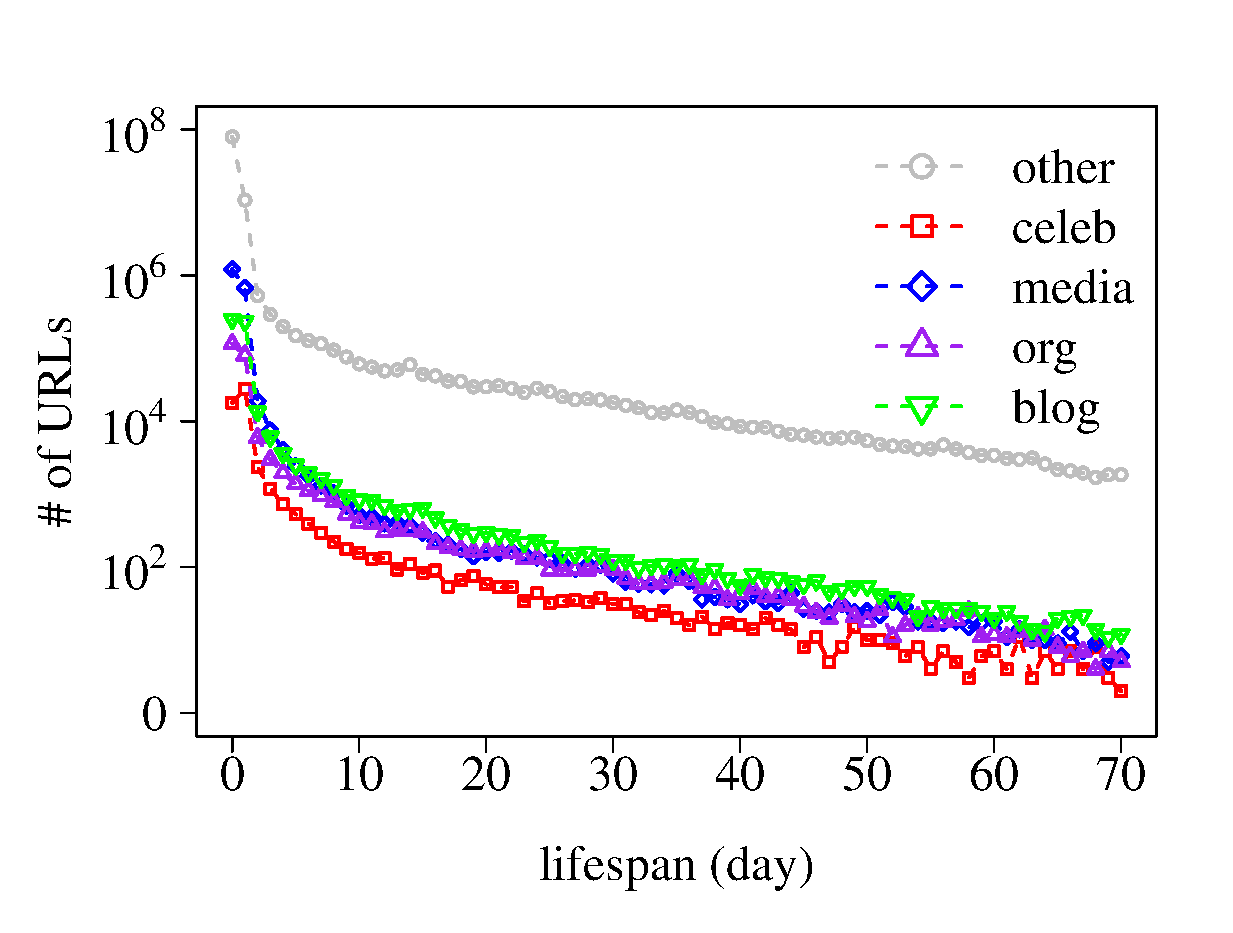
\includegraphics[width=3in]{figures/url_lifespan_by_categories_500K_censored.eps}
\caption{Histogram of lifespan of URLs originating from different categories}
\label{fig:lifespan_category}
\end{figure}

\begin{figure}
\centering
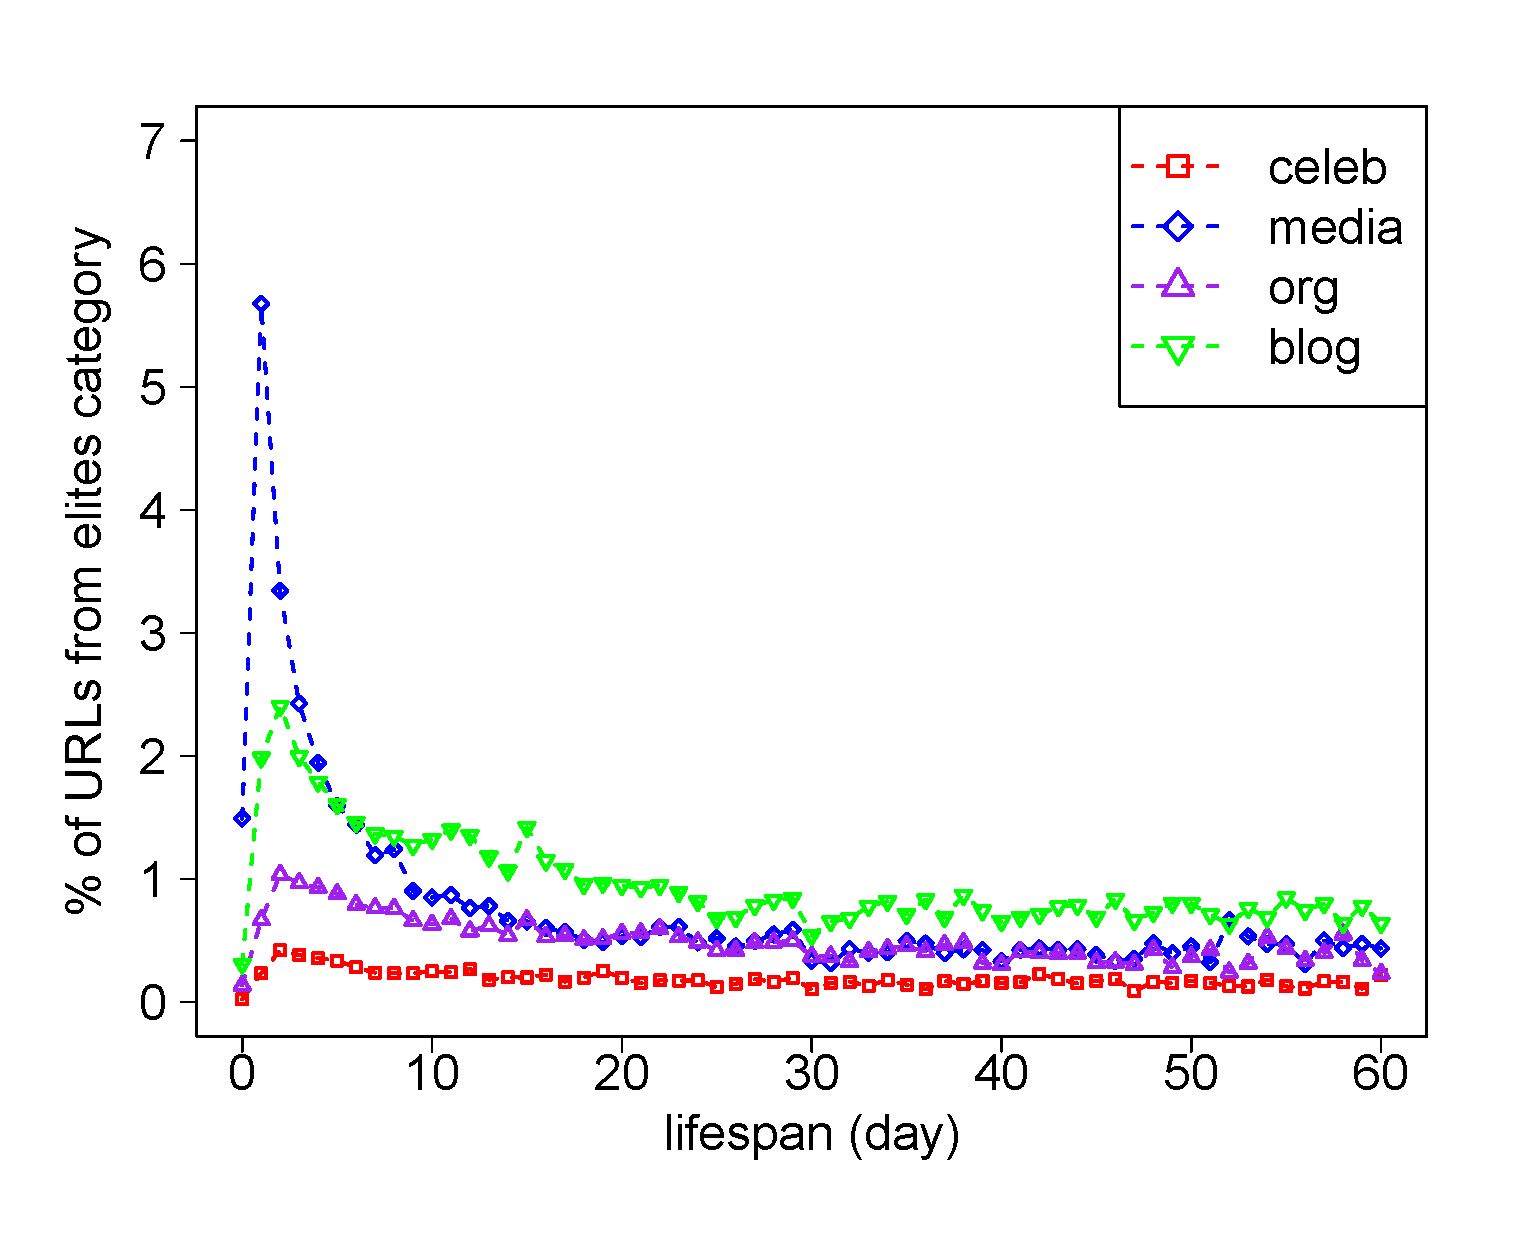
\includegraphics[width=3in]{figures/url_lifespan_percentage_by_categories_500K_censored.eps}
\caption{Percentage of URL initiated by 5 categories, with different lifespan}
\label{fig:lifespan_percentage_category}
\end{figure}


A second related point, is illustrated by Figure
\ref{fig:RT_lifespan_category}, which shows the average RT rate = (\# of
retweets) / (total \# of occurrences) of URLs with different lifespan,
grouped by categories\footnote{Note here that URLs with lifespan = 0 are
  those URLs that only appeared once in our dataset, thus the RT rate is
  zero.}. 
%
Unsurprisingly, URLs introduced by elite users are much more likely than
those introduced by ordinary users to be RT'd---a result that is likely
driven by the higher-than-average number of followers for elite users.
Somewhat less expected, however, is that for all categories the majority of
appearances of URLs after their initial introduction derives not from
rebroadcasting, hence diffusion within Twitter, but rather from
reintroduction. As large and diverse as Twitter is, in other words, it is
nevertheless a subset of a much larger media ecosystem; that is, content
``lives'' outside of Twitter, where users can rediscover it
repeatedly. Some of this content---such as daily news stories---has a
relatively short period of relevance, after which a given story is unlikely
to be reintroduced or rebroadcast. At the other extreme, classic music
videos, movie clips, and long-format magazine articles have lifespans that
are effectively unbounded, and can be rediscovered and reintroduced by
Twitter users indefinitely without losing relevance.

\begin{figure}
\centering
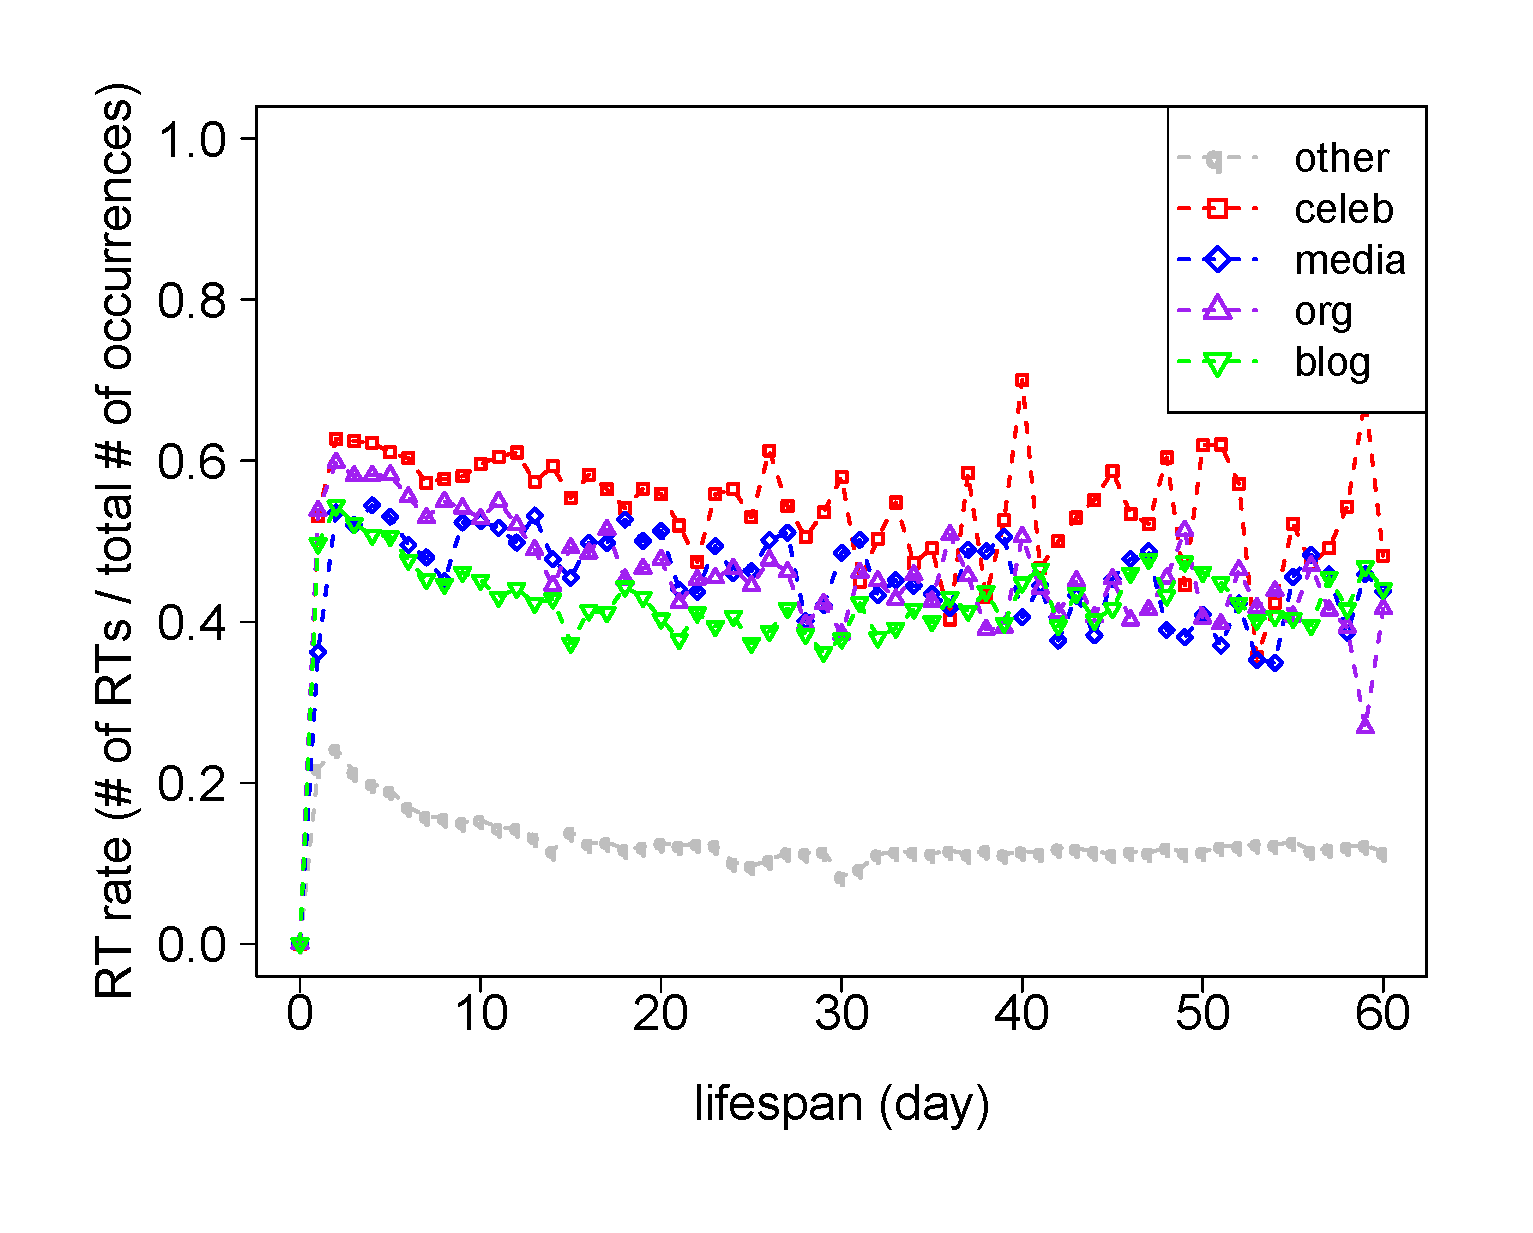
\includegraphics[width=3in]{figures/url_lifespan_RTrate_by_categories_500K_censored.eps}
\caption{Lifetime ~ avg RT rate, by categories}
\label{fig:RT_lifespan_category}
\end{figure}

To shed more light on the nature of long-lived content on Twitter, we used
the bit.ly API service to unshorten 35K of the most long-lived URLs (URLs
that lived at least 200 days), and mapped them into 21034 web domains. As
Figure \ref{fig:longlived_urls} shows, the population of long-lived URLs is
dominated by videos, music, and books, consistent with our interpretation
above that certain types of online content retain their relevance
indefinitely, and their persistence on Twitter is driven mostly by users
rediscovering content outside of the Twitter ecosystem.

\begin{figure}
\centering
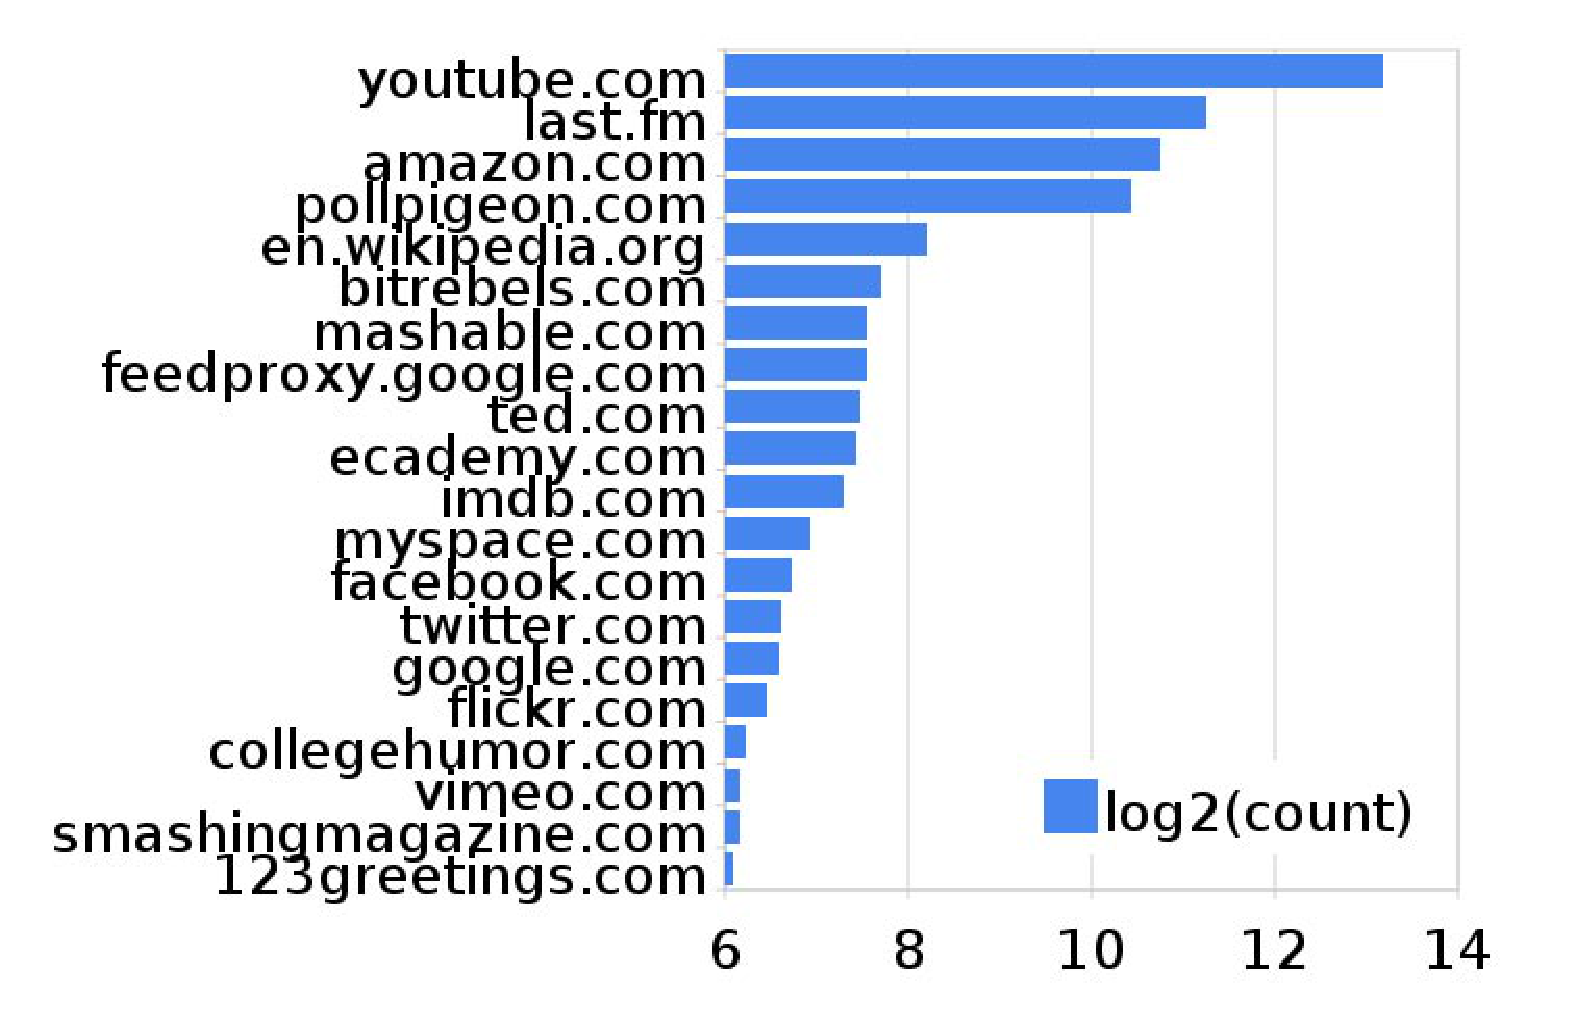
\includegraphics[width=3in]{figures/domains_breakdown_longlived_urls.eps}
\caption{Top 20 domains for URLs that lived more than 200 days}
\label{fig:longlived_urls}
\end{figure}

% \subsection{Predicting Lifetime} 
%
% Although the previous analysis shows that URLs initiated by certain types
% of users have higher-than-average retweet rates, and that certain types
% of content are overrepresented among long-lived URLs, it does not
% necessarily follow that one can predict either the success or lifespan of
% a URL with much confidence. Bakshy et al. \cite{bakshy_11}, for example,
% found that although large cascades tend to be initiated by users with
% large $\#$ followers and successful track records, most instances of URLs
% introduced by users with those attributes do not generate large cascades.
% Here we find a similar result.

%% Describe model and results.


\subsection{Content}

Informatoin filtering does not mean high interpersonal influence. The persistence of long-last content can not be fully contributed to contagion process - the role of content. 

Evidence: RT rate for information with different lifespan. 

Role of content? Domain breakdown.

\subsubsection{Data}
To study content in more details, we introduce a smaller Twitter dataset with richer HTML content. 

\subsubsection{Relationship between content and persistence}
Strong collrection between content and the persistence of information.

\subsection{Negative influence}

\subsubsection{Data}
Orkut: social network with detailed structure, spread of behavior.


\chapter{Answer social science questions with social media data}
\section{Lasswell's Maxim}

\section{Two-step flow}

\section{Social movement}


\chapter{the interaction between people and information}

In~\cite{Wu-Twitter-2011}, we studied the production, flow, and consumption of information in Twitter. As suggested in previous research in public communications, we classified users into 5 categories (celebrities, bloggers, mass media, organizations, and others) and found a striking concentration of attention on a small number of ``elite'' users on Twitter, as well as a significant homophily within categories. We also applied the classical ``two-step flow'' theory of communications in the context of social media sites such as Twitter. Our results confirmed that there are a large number of intermediary users who actively filter and disseminate information from media to the masses, and the composition of intermediaries is highly diverse. We also examined the lifespan and content of URLs broadcasted by different categories of users. We found that although content picked up by bloggers tends to stimulate a more persistent interest, the longevity of information is determined not by diffusion process, but by many different users independently rediscovering the same content.




\chapter{the role of content}
Following up our previous work, in~\cite{Wu-ICWSM-2011}, we studied the relationship between content and the temporal dynamics of information on Twitter, focusing on the persistence of information. Our results demonstrated a strong association between the content and the temporal dynamics of information. For example, rapidly-fading information contains significantly more words related to negative emotion, actions, and more complicated cognitive processes, whereas persistent information contains more words related to positive emotion, leisure, and lifestyle.

\chapter{Network effect and behavioral contagion}

\chapter{Diffusion without active dissemination}

Arrival and Departure Dynamics in Online Social Networks (submitted to the International Conference on Web Wide Web, 2012). 

In this paper, we compared the dynamics of user arrival and departure in online social networks. We showed although user disengagement has been considered less viral than engagement, there is a substantial network effect of the departure of friends on a user's tendency to leave a network. Taking into account such network effect, we are able to build machine learning models to predict the departure of users based on their local network properties.


\chapter{Social media in Arab Spring Movement}
    Joining social media data with real world events, we are able to study one of the most interesting (and also the most difficult) parts in media communication research (Lasswell's maxim): the effect of information. One of my ongoing projects is to study the role of social media in social movements, in order to understand how the propagation of information is leading or reflecting societal changes. We have collected a large number of tweets and twitter networks related to big social movements (i.e., Middle East Revolution, Occupy WallStreet Movement). Using effective algorithms for community detection, hub detection, trend detection, and opinion mining, we will be able to identify the informal structure of massive communication networks for social movements and study the diffusion of ideology and behaviors within and across organizational/geographical boundaries.


\section{Data}
To collect a substantial set of users and their tweets from the Middle East area in the period of the recent social movements, we first identified a set of countries of interest, including Tunisia, Egypt, Libya, Bahrain, Iran, Iraq, Israel, Algeria, Morocco, Saudi Arabia, Kuwait, Yemen, United Arab Emirates, Palenstine, Quatar, Oman, Jordan, Cyprus, Syria, and Lebanon. For each country, we used Yahoo Maps APIs to get the list of cities and towns in that country, together with the geographical centroid point for each city/town, in the form of (latitude, longitude).

After we had the centroid points of cities/towns within a country, we used Twitter search APIs to retrieve all the recent tweets generated within 100 miles from every centroid point in that country. We then parsed these tweets and extracted the authors of these tweets.

Using these authors as ``seeds'', we crawled one degree out from the seeds, and retrieved the profiles of all the seeds, and all the neighbors (friends/followers) of the seeds. The size of graph grows rapidly in one-degree distance. In fact, the network induced by the seeds and their one-degree neighbors already cover over 3 millions distinct Twitter users.

We crawled the profiles of these 3M users, and tried to identify their country of origin in three ways:
\begin{enumerate}
\item look for the country name in their self-reported location in their profile;
\item if the time-zone city is specified in their profile, map the city to the corresponding country;
\item if the location-tracking service is turned on, get the tracked location in Twitter meta data.
\end{enumerate}

After parsing the profiles for all 5M users, we were able to identify the country of origin for 260K of them.

In the end, we crawled the maximal available history of tweets generated by these $260K$ users, which is, up to $3200$ tweets per user. In the end we collected in total $96,350,865$ tweets in this way. Among them, 36,857,387 were generated between Dec 1st, 2010 and March 31st, 2011, by 112,661 users  from the countries listed above.

Here is a breakdown of the amount of data we collected from each country.

To compare the diffusion of protest and non-protest content on Twitter, we first identify protest-related tweets. We say a tweet is related to protest if it contains at least one protest hashtag .  Protest hashtags are hand-picked by political scientists. However, as there are hundreds of thousands of  hashtags in our dataset, it is not feasible for political scientists to manually label all the hashtags. To effectively identify protest-related hashtags while maintaining a high recall, we narrow the pool of hashtags to be examined based on two metrics: (1) the volume of tweets containing the hashtag; and (2) the bursty-ness (as defined by Kleinberg 2004 KDD) of the hashtag occurrence. In this way, we narrow the scope down to only the top 1000 most frequently used hashtags and the top 1000 most bursty hashtags. We then have the experts to only go through those 2000 hashtags, and are able to identify about 500 protest-related hashtags among them.

\section{Method and Results}
As shown in the previous section, there had been a substantial amount of protest content introduced by Egyptian users on Twitter, even before Jan 25, 2011, when the first big protests took place in Tahrir Square, Cairo. Who were V those foresighted users? Were they planning and organizing the protests? Were  they qualitatively different than other users on Twitter? In this section, we will investigate these questions, focusing on the relationship between the status of users and their earliness at participating in the protest activities on Twitter.

To start, we first represent the earliness of a user by his mobilization day. A user u's mobilization day d(u), is defined as the day when u first used any protest hashtag. We then quantify the status of user u on day t,  by the number of Twitter followers u has on day t. In order to show the aggregated status of users who started to participate in the protest at different times, we group users by their mobilization day d, and calculate f(d), the median value of user status, for each group. In Figure 4, we plot f(d) for d between December 10, 2010 and January 25, 2011. Here we can see a clear trend of decreasing status as the mobilization day gets  closer to the actual protest day.

\section{Conclusion}
By analyzing Twitter activity in Middle East area during the Arab Spring movement, we have shown that social media were used to both activate and reflect the on-goings of Middle East social movement. The relative weights of these two roles differed across countries. In particular, Egyptian users actively used Twitter to plan protests and call for a critical mass, and the users from Saudi Arabia or UAE mostly used Twitter to support or comment on on-going events. We also found that protest content travelled directionally from the central to the peripheral of the Twitter network:  most protest memes were initiated by hub users and later picked up by the masses.  At the individual level, we found that the adoption of protest content can be modeled by the complex contagion process - while the overall adoption rate of protest content is relatively low, people become significantly more likely to start tweeting about the protest when more than 2 friends already doing so. 

 Although our work is to our best knowledge the largest study of the role of social media in social movements, we have to acknowledge that our dataset is rather disproportionate: $80\%$ of the tweets we studied came from only 5 Middle East countries. Due to technical issues, we were not able to collect an equally large number of tweets from countries such as Libya, Tunisia, and Algeria, when dramatic societal changes were taking places in these countries.

For the future work, we want to extend our study to the diffusion of protest content among countries and communities through social media. Another interesting direction is to understand how mass media (newspaper, TV, radio) and social media interact and influence each other in social movements.

This work presents one of the largest studies on the role of social media in the Arab Spring movement. Using over 2 million tweets generated by 110 thousand users in 11 Middle East countries during early 2011, we depict the landscape of aggregated Twitter usage in those countries as the revolution unfolded. Our results suggest that social media has been used to both lead and reflect real world protest activities. Compared to non-protest-related content on Twitter, we find that protest-related content travels directionally from central users to peripheral users, and the adoption of protest-related content can be modeled by a complex contagion process. 

\chapter{Conclusion}
    In summary, I am deeply intrigued by the developing characteristics of information diffusion in online social media. Thanks to the Internet and social media technologies, I believe that we are heading towards a more democratic era where revolutions can be started by ordinary people and the power to change is in the hands of the masses. As part of this process, social media sites such as Facebook and Twitter have also evolved from friendship networks to a much broader platform for organizing social/political changes and communicating with various communities. I hope my work can help understand this movement and foster the effective flow of information in the society.


\appendix
\chapter{Chapter 1 of appendix}
Appendix chapter 1 text goes here

\bibliography{diffusion}

\end{document}
